\chapter{Policy-based RL}
\label{sec:policySearch}



%https://lilianweng.github.io/lil-losg/2018/04/08/policy-gradient-algorithms.html

In the previous section, we considered methods that
estimate the action-value function, $Q(s,a)$,
from which we derive a policy.
%If $Q$ is close to $\Qopt$,
%the resulting policy will be near optimal.
%e.g., $\policy(a|s)=\ind{a=\argmax_a Q(s,a)}$
%or $\policy(a|s) = e^{Q(s,a)}/\sum_{a'} e^{Q(s,a')}$.
However, these methods have several disadvantages:
(1)  they can be difficult to apply to continuous action spaces;
(2) they may diverge if function approximation is used (see
\cref{sec:deadlyTriad});  
(3) the training of $Q$, often based on TD-style updates,
is not directly related to the expected return
garnered by the learned policy;
(4) they learn deterministic policies,
whereas in stochastic and partially observed environments,
stochastic policies are provably better
\citep{Jaakkola94}.

In this section, we discuss
\keywordDef{policy search} methods,
which directly optimize the parameters of the policy
so as to maximize its expected return.
We mostly focus on \keywordDef{policy gradient} methods,
that use the gradient of the loss to guide the search.
As we will see,  these policy methods often 
benefit from estimating a value or advantage function
to reduce the variance in the policy search process,
so we will also use techniques from \cref{sec:valueRL}.
The parametric policy will be denoted by 
$\pi_{\vtheta}(a|s)$.
For discrete actions, this can be a DNN with a softmax output.
For continuous actions, we can use a Gaussian output layer,
or a diffusion policy \citep{Ren2024}.

For more details on policy gradient methods, see \citep{weng2018PG,Lehmann2024}.



\eat{
\footnote{
%
To handle multimodal distributions, it has recently
become popular to use more expressive policy classes such as diffusion
models;
this is known as a \keywordDef{diffusion policy}
\citep{diffusionPolicy}.
However, since it is difficult to compute the probability
value of the output from diffusion, such models are usually
trained using behavior cloning (\cref{sec:BC}),
rather than the policy gradient methods we discuss in this section.
%(For a recent survey of other ways to apply diffusion in RL,
%see \citep{diffusionRL}.)
}
}

\section{The policy gradient theorem}
\label{sec:policyGradient}
\label{sec:PG}


%http://timvieira.github.io/blog/post/2019/04/20/the-likelihood-ratio-gradient/

We start by defining the objective function
for policy learning,
and then derive its gradient.
%We consider the episodic case.
%A similar result can be derived for the continuing case with the average reward
%criterion~\citep[Sec 13.6]{Suttonv2}.
The objective, which we aim to maximize, is defined as
\begin{align}
  J(\pi)  &\defeq \expectQ{\sum_{t=0}^{\infty} \gamma^t R_{t+1}}{\pi} \\
  &= \sum_{t=0}^{\infty} \gamma^t \sum_s \left(\sum_{s_0}
  p_0(s_0) p^{\pi}(s_0 \rightarrow s, t) \right)
  \sum_a \pi(a|s) R(s,a) \\
  &= \sum_s 
  \left(
  \sum_{s_0} \sum_{t=0}^{\infty} \gamma^t 
  p_0(s_0) p^{\pi}(s_0 \rightarrow s, t) \right)
  \sum_a \pi(a|s) R(s,a) \\
  &= \sum_s \rho^{\pi}(s)    \sum_a \pi(a|s) R(s,a) 
\end{align}
where we have defined the discounted state visitation
measure
\be
\statmeasure_{\pi}^{\gamma}(s) \defeq
\sum_{t=0}^{\infty} \gamma^t
\underbrace{\sum_{s_0}   p_0(s_0) p^{\pi}(s_0 \rightarrow s, t)}_{p_t^{\pi}(s)}
\ee
where
$p^{\pi}(s_0 \ra s, t)$ is the probability of going
from $s_0$ to $s$ in $t$ steps,
and
$p_t^{\pi}(s)$ is the marginal probability of being in state $s$
at time $t$ (after each episodic reset).
Note that $\statmeasure_{\pi}^{\gamma}$ is a measure of time spent in  non-terminal states,
but it is not a probability measure, since it is not normalized,
i.e., $\sum_s \statmeasure_{\pi}^{\gamma}(s) \neq 1$.
However, we may abuse notation and still treat it like a probability,
so we can write things like
\be
\expectQ{f(s)}{\statmeasure_{\pi}^{\gamma}(s)} =
\sum_s \statmeasure_{\pi}^{\gamma}(s) f(s)
\ee
Using this notation, we can define the objective as
\be
J(\pi) = \expectQ{R(s,a)}{\statmeasure_{\pi}^{\gamma}(s), \pi(a|s)}
\label{eqn:JJpi}
\ee
We can also define a normalized version of the measure $\statmeasure$
by noting that
$\sum_{t=0}^{\infty} \gamma^t = \frac{1}{1-\gamma}$ for $\gamma<1$.
Hence the normalized discounted state visitation distribution
is given by
\be
\statdistpol(s) = (1-\gamma) \statmeasure_{\pi}^{\gamma}(s)
= (1-\gamma) \sum_{t=0}^{\infty} \gamma^t p_t(s)
\label{eqn:statdistpol}
\ee
(Note the change from $\rho$ to $p$.)

Note that in 
\citep[Sec 13.2]{Suttonv2}, they use slightly different notation.
In particular, they assume $\gamma=1$,
and define the non-discounted state visitation measure
as $\eta(s)$ and the corresponding normalized version by $\mu(s)$.
This is equivalent to ignoring  the discount factor $\gamma^t$
when defining $\statmeasure_{\pi}(s)$.
This is standard practice in many implementations,
since we can just average over (unweighted)
trajectories when estimating
the objective and its gradient,
even though it
results in a biased estimate
\citep{Nota2020,Che2023}.

It can be shown that the gradient of the above objective is
given by
\begin{align}
\nabla_{\vtheta} J(\vtheta)
&=\sum_s \statmeasure_{\pi}^{\gamma}(s)
\sum_a Q^{\pi}(s,a) \nabla_{\vtheta} \pi_{\vtheta}(a|s)
\label{eqn:PGthm}
\\
&=\sum_s \statmeasure_{\pi}^{\gamma}(s)
\sum_a Q^{\pi_{\vtheta}}(s,a) \pi_{\vtheta}(a|s) \nabla_{\vtheta} \log \pi_{\vtheta}(a|s) \\
&=\expectQ
{Q^{\pi_{\vtheta}}(s,a) \nabla_{\vtheta} \log \pi_{\vtheta}(a|s)}
    {\statmeasure_{\pi}^{\gamma}(s) \pi_{\vtheta}(a|s)} 
\label{eqn:SFE}
\end{align}
This is known as the \keywordDef{policy gradient theorem}
\citep{Sutton99b}.
In statistics, the term $\nabla_{\vtheta} \log \pi_{\vtheta}(\va|\vs)$
is called the (Fisher) \keywordDef{score function}\footnote{
%
This is distinct from the Stein score,
which is the gradient wrt the argument of the log probability,
$\nabla_{\va} \log \pi_{\vtheta}(\va|\vs)$,
as used in diffusion.
},
so sometimes \cref{eqn:SFE}
is called the \keywordDef{score function estimator}
or \keywordDef{SFE} \citep{Fu2015,Mohamed2020}.



\section{REINFORCE}
\label{sec:REINFORCE}
\label{sec:reinforceOpt}
\label{sec:reinforce}

% Pieter Abeel lecture notes
%https://drive.google.com/file/d/0BxXI_RttTZAhY216RTMtanBpUnc/view


% Sutton p327
One way to apply the policy gradient theorem
to optimize a policy is to use stochastic gradient ascent.
Theoretical results concerning the convergence
and sample complexity of such
methods can be found in \citep{Agarwal2021}.

To implement such a method,
let
$\traj=(s_0,a_0,r_0,s_1,\ldots,s_T)$ be
a trajectory created by sampling from $s_0\sim\initdist$
and then following $\polapprox$.
Then we have
\begin{align}
\nabla_{\vtheta} \polval(\polapprox)
&=
\sum_{t=0}^{\infty} \gamma^t \expectQ{
  \nabla_{\vtheta} \log \polapprox(a_t|s_t) \Qpolapprox(s_t,a_t)}
    {p_t(s) \polapprox(a_t|s_t)} \\
  &\approx \sum_{t=0}^{T-1} \gamma^t \return_t \nabla_{\vtheta} \log\polapprox(a_t|s_t)
\end{align}
where the return  is defined as follows
\begin{align}
\return_t &\defeq r_t + \gamma r_{t+1} + \gamma^2 r_{t+2} + \cdots
+ \gamma^{T-t-1} r_{T-1} 
= \sum_{k=0}^{T-t-1} \gamma^k r_{t+k}
= \sum_{j=t}^{T-1} \gamma^{j-t} r_j
\end{align}
See \cref{algo:REINFORCE} for the pseudocode.

\begin{algorithm}
\dontprintsemicolon
\caption{REINFORCE (episodic version)}
\label{algo:REINFORCE}
Initialize policy parameters $\vtheta$\\
\Repeat{converged}
       {
         Sample an episode $\traj=(s_0, a_0, r_0, s_1, \ldots, s_T)$ using $\polapprox$ \\
         %Compute $\return_t$ for all $t\in\{0,1,\ldots,T-1\}$ using \cref{eqn:rl-return} \\
         \For{$t=0,1,\ldots,T-1$}{
           $\return_t = \sum_{k=t+1}^T \gamma^{k-t-1} R_k$ \\
           $\vtheta \assign \vtheta + \lr_{\vtheta} \gamma^t \return_t
           \nabla_{\vtheta} \log \policy_{\vtheta}(a_t|s_t)$
         }
}
\end{algorithm}

In practice, estimating the policy gradient using
\cref{eqn:SFE} can have a high variance.
A \keywordDef{baseline} function $b(s)$ can be used for variance reduction
to get
\begin{align}
\nabla_{\vtheta} \polval(\polapprox) = 
 \expectQ{\nabla_{\vtheta} \log \polapprox(a|s) (\Qpolapprox(s,a) - b(s))}
{\statmeasure_{\vtheta}(s) \polapprox(a|s)}
\label{eqn:PGthmBaseline}
\end{align}
Any function that satisfies $\expect{\nabla_{\vtheta} b(s)}=0$ is a valid
baseline.
This follows since
\be
\sum_a  \nabla_{\vtheta} \pi_{\vtheta}(a|s) (Q(s,a)-b(s))
= \nabla_{\vtheta} \sum_a \pi_{\vtheta}(a|s) Q(s,a)
-\nabla_{\vtheta} [\sum_a \pi_{\vtheta}(a|s)] b(s)
= \nabla_{\vtheta} \sum_a \pi_{\vtheta}(a|s) Q(s,a) - 0
\ee
A common choice for the baseline is $b(s) = \Vpolapprox(s)$.
This is a good choice since $\Vpolapprox(s)$ and $Q(s,a)$ are correlated
and have similar magnitudes,
so the scaling factor in front of the gradient term will be small.
%(See also \citep{Wu2018} for an action-dependent baseline.)

Using this we get an update of the following form
\begin{align}
  \vtheta \assign \vtheta + \lr \sum_{t=0}^{T-1}
  \gamma^t (G_t - b(s_t)) \nabla_{\vtheta} \log\polapprox(a_t|s_t)
\label{eqn:REINFORCE}
\end{align}
This is 
is called the \keywordDef{REINFORCE} estimator
\citep{Williams1992}.\footnote{
  %
  The term 
``REINFORCE'' is an acronym for
``REward Increment = nonnegative Factor x Offset
Reinforcement x Characteristic Eligibility''.
The phrase ``characteristic eligibility'' refers to  the
$\nabla \log \polapprox(a_t|s_t)$ term;
the phrase ``offset reinforcement'' refers to the
$\return_t-b(s_t)$ term;
and the phrase ``nonnegative factor''
refers to the learning rate $\lr$ of SGD.
} %
The update equation
 can be interpreted as follows:
we compute the sum of discounted future rewards
induced by a trajectory, compared to a
baseline,  and if this is positive, we increase
$\vtheta$ so as to make this trajectory more likely,
otherwise we decrease $\vtheta$.
Thus, we reinforce good behaviors,
and reduce the chances of generating bad ones.



\eat{
\cref{algo:REINFORCEbaseline} gives the pseudocode
where we use  separate learning rates
for the two objectives.

\begin{algorithm}
\dontprintsemicolon
\caption{REINFORCE (episodic) with value function baseline}
\label{algo:REINFORCEbaseline}
Initialize policy parameters $\vtheta$, baseline parameters $\vw$\\
\Repeat{converged}
       {
         Sample an episode $\traj=(s_0, a_0, r_0, s_1, \ldots, s_T)$ using $\polapprox$ \\
         %Compute $\return_t$ for all $t\in\{0,1,\ldots,T-1\}$ using \cref{eqn:rl-return} \\
         \For{$t=0,1,\ldots,T-1$}{
           $\return_t = \sum_{k=t+1}^T \gamma^{k-t-1} R_k$ \\
           $\delta_t = \return_t - \Vapprox(s_t)$  \\
           $\vw \assign \vw - \lr_{\vw} \delta_t \nabla_{\vw}
           \Vapprox(s_t)$  \\
           $\vtheta \assign \vtheta + \lr_{\vtheta} \gamma^t \delta_t
           \nabla_{\vtheta} \log \policy_{\vtheta}(a_t|s_t)$ 
         }
}
\end{algorithm}
}


\section{Actor-critic methods}
\label{sec:actorCritic}
\label{sec:AC}



An \keywordDef{actor-critic} method \citep{Barto1983}
uses the policy gradient method,
but where the expected return $G_t$ is estimated
using temporal difference learning
of a value function instead of MC rollouts.
(The term ``actor'' refers to the policy,
and the term ``critic'' refers to the value function.)
The use of bootstrapping in TD updates
allows more efficient learning of the value function
compared to MC, and further reduces the variance.
In addition, it allows us to develop a fully online, incremental
algorithm, that does not need to wait until the end of the trajectory
before updating the parameters.


\subsection{Advantage actor critic (A2C)}
\label{sec:A2C}
\label{sec:A3C}

% Sutton p331
Concretely, consider the use of the one-step TD method
to estimate the return in the episodic case,
i.e., we replace $\return_t$ with
$\return_{t:t+1}=r_t+ \gamma \Vapprox(s_{t+1})$.
If we use $\Vapprox(s_t)$ as a baseline,
the REINFORCE update in \cref{eqn:REINFORCE} becomes
\begin{align}
\vtheta 
&\assign \vtheta + \lr \sum_{t=0}^{T-1} \gamma^t \left(G_{t:t+1} - \Vapprox(s_t)\right) \nabla_{\vtheta} \log\polapprox(a_t|s_t) \\
&= \vtheta + \lr \sum_{t=0}^{T-1} \gamma^t \big(r_t+ \gamma \Vapprox(s_{t+1}) - \Vapprox(s_t)\big) \nabla_{\vtheta} \log\polapprox(a_t|s_t)
\end{align}

%This  can be extended to the off-policy
%setting as explained in e.g., \citep{Degris2012,Zhang2019}.
%https://medium.com/@jonathan_hui/rl-policy-gradients-explained-advanced-topic-20c2b81a9a8b



Note that
$\delta_t = r_{t+1} + \gamma \Vapprox(s_{t+1}) -\Vapprox(s_t)$
is a single sample approximation
to the advantage function $A(s_t,a_t) = Q(s_t,a_t) - V(s_t)$.
%We can alternatively learn the advantage function
%directly, and use $A(s_t,a_t)$ instead
%of $\return_{t:T}$ (as in vanilla REINFORCE),
%or $\return_t^{(1)}$ (as in REINFORCE with a TD(0) baseline).
This method is therefore called 
\keywordDef{advantage actor critic} or \keywordDef{A2C}.
See \cref{algo:A2C} for the pseudo-code.\footnote{
%
In \citep{A3C}, they proposed
a distributed version of A2C known as
\keywordDef{A3C} 
which stands for  ``asynchrononous advantage actor critic''. 
}
(Note that $V_{\vw}(s_{t+1})=0$ if $s_t$ is a done state,
representing the end of an episode.)
Note that this is an on-policy algorithm,
where we update the value function $V_{\vw}^{\pi}$
to reflect the value of the current policy $\pi$.
See \cref{sec:bilevel} for further discussion of this point.

% https://github.com/DLR-RM/stable-baselines3/blob/master/stable_baselines3/a2c/a2c.py


\begin{algorithm}
\dontprintsemicolon
\caption{Advantage actor critic (A2C) algorithm (episodic)}
\label{algo:A2C}
Initialize actor parameters $\vtheta$, critic parameters $\vw$\\
\Repeat{converged}
       {
       Sample starting state $s_0$ of a new episode \\
       \For{$t=0,1,2,\ldots$}
       {
         Sample action $a_t \sim \polapprox(\cdot|s_t)$ \\
         $(s_{t+1},r_t,\done_t) = \text{env.step}(s_t,a_t)$ \\
        $\targetV_t = r_t + \gamma (1-\done_t) \Vapprox(s_{t+1})$       // Target \\
       $\delta_t = \targetV_t - \Vapprox(s_t)$ // Advantage \\
           $\vw \assign \vw  + \lr_{\vw} \delta_t \nabla_{\vw}
       \Vapprox(s_t)$ // Critic \\
           $\vtheta \assign \vtheta + \lr_{\vtheta} \gamma^t \delta_t
       \nabla_{\vtheta} \log \polapprox(a_t|s_t)$ // Actor \\
       \If{$\done_t=1$}{break}
         }
}
\end{algorithm}

In practice, we should use a stop-gradient
operator on the target value for the TD update,
for reasons  explained in \cref{sec:deadlyTriad}.
Furthermore, it is common to add an entropy term
to the policy, to act as a regularizer
(to ensure the policy remains stochastic, which smoothens
the loss function --- see \cref{sec:SAC}).
If we use a shared network with separate value  and policy heads,
we need to use a single loss function for training all the parameters
$\vphi$.
Thus we get the following loss, for each trajectory,
where we want to minimize TD loss,
maximize the policy gradient (expected reward) term,
and maximize the entropy term.
\begin{align}
  \loss(\vphi;\tau) &= \frac{1}{T} \sum_{t=1}^T \left[
    \lambda_{TD} \loss_{TD}(s_t,a_t,r_t,s_{t+1})
    -    \lambda_{PG} J_{PG}(s_t,a_t,r_t,s_{t+1})
    -    \lambda_{ent} J_{ent}(s_t)
    \right]
  \label{eqn:ACloss}\\
  \targetV_t &= r_t + \gamma (1-\done(s_t)) V_{\vphi}(s_{t+1}) \\
  \loss_{TD}(s_t,a_t,r_t,s_{t+1})  &= (\stopgrad(\targetV_t) - V_{\phi}(s))^2 \\
  J_{PG}(s_t,a_t,r_t,s_{t+1}) &= (\stopgrad(\targetV_t - V_{\phi}(s_t))
  \log \pi_{\vphi}(a_t|s_t) \\
  J_{ent}(s_t) &= -\sum_a \pi_{\vphi}(a|s_t) \log \pi_{\vphi}(a|s_t)
\end{align}
To handle the dynamically varying scales of the different loss functions,
we can use 
the \keywordDef{PopArt} method
of \citep{van-Hasselt2016,Hessel2019}
to allow for a fixed set of hyper-parameter values for $\lambda_i$.
(PopArt  stands for
``Preserving Outputs Precisely, while Adaptively Rescaling Targets''.)

\eat{
\begin{align}
  \loss(\vphi;\tau) = \frac{1}{T} \sum{t=1}^T \left[
    \lambda_{TD} (\stopgrad(\targetV_t) - V_{\vphi}(\vs_t))^2
    -    \lambda_{PG} (\stopgrad(\targetV_t - V_{\vphi}(\vs_t))
    -    \lambda_{ent} \entropy(\pi_{\vphi}(\cdot|\vs_t))
    \right]
  \end{align}
}

\eat{
We can then accumulate  the following gradients
over each sampled trajectory:
\begin{align}
  \nabla_{\vw}  &= -\frac{1}{2T} \sum_t
  \nabla_{\vw} (\targetV_t - V_{\vw}(s_t))^2 
  = \frac{1}{T} \sum_t  (\targetV_t - V_{\vw}(s_t)) \nabla_{\vw} V_{\vw}(s_t) \\
  \nabla_{\vtheta} &= \frac{1}{T} \sum_t
  (\targetV_t - V_{\vw}(s_t)) \nabla_{\vtheta} \log \pi_{\vtheta}(a_t|s_t)
  \end{align}
The second gradient ignores the discount term $\gamma^t$,
but omitting this is standard practice,
even though it
results in a biased estimate
\citep{Nota2020,Che2023}.
}


\eat{
For a more practical minibatch version,
based on \citep{Ivanov2019},
see \cref{algo:A2C}.
}

\subsection{Generalized advantage estimation (GAE)}
\label{sec:GAE}

%\subsection{AC with $n$-step critics}

In A2C, we replaced the high variance, but unbiased,
MC return $G_t$
with the low variance, but biased,
one-step bootstrap return $G_{t:t+1} = r_t + \gamma V_{\vw}(s_{t+1})$.
More generally, we can compute the
$n$-step estimate
\begin{align}
G_{t:t+n} =
r_t + \gamma r_{t+1} + \gamma^2 r_{t+2}
+ \cdots + \gamma^{n-1} r_{t+n-1} + \gamma^n \Vapprox(s_{t+n})
\end{align}
and thus obtain  the (truncated) $n$-step advantage estimate as follows:
\be
A_{\vw}^{(n)}(s_t,a_t) = G_{t:t+n} - \Vapprox(s_t)
\ee
Unrolling to infinity, we get
% https://nn.labml.ai/rl/ppo/gae.html
\begin{align}
  A_t^{(1)} &= r_t + \gamma v_{t+1} - v_t  \\
  A_t^{(2)} &= r_t + \gamma r_{t+1} + \gamma^2 v_{t+2} - v_t  \\
  &\vdots \\
  A_t^{(\infty)} &= r_t + \gamma r_{t+1} + \gamma^2 r_{t+2} +\cdots - v_t 
  \end{align}
$A_t^{(1)}$ is high bias but low variance,
and $A_t^{(\infty)}$  is unbiased but high variance.


%https://nn.labml.ai/rl/ppo/gae.html
% https://github.com/google-deepmind/rlax/blob/master/rlax/_src/multistep.py#L39
% https://github.com/EdanToledo/Stoix/blob/main/stoix/utils/multistep.py#L12
% https://github.com/luchris429/purejaxrl/blob/main/purejaxrl/ppo.py#L142
%https://github.com/DLR-RM/stable-baselines3/blob/master/stable_baselines3/common/buffers.py#L402

Instead of using a single value of $n$, we can take
a weighted average.
That is, we define
\be
A_t = \frac{\sum_{n=1}^T w_n A_t^{(n)}}{\sum_{n=1}^T w_n}
\ee
If we set $w_n = \lambda^{n-1}$ we get the following simple recursive
calculation:
\begin{align}
  \delta_t &= r_t + \gamma v_{t+1} - v_t \\
  A_t &= \delta_t + \gamma \lambda \delta_{t+1} + \cdots +
  (\gamma \lambda)^{T-t+1} \delta_{T-1} = \delta_t + \gamma \lambda
  A_{t+1}
  \end{align}
Here $\lambda \in [0,1]$ is a parameter that controls the bias-variance
tradeoff: larger values decrease the bias but increase the variance.
This is called \keywordDef{generalized advantage estimation}
(\keywordDef{GAE})~\citep{GAE}.
See \cref{algo:GAE} for some pseudocode.
Using this, we can define a general actor-critic
method, as shown in \cref{algo:AC}.

\begin{algorithm}
\dontprintsemicolon
\caption{Generalized Advantage Estimation}
\label{algo:GAE}
$\text{def GAE}(r_{1:T},v_{1:T}, \gamma, \lambda)$\\
$A'=0$ \\
\For{$t=T:1$}{
  $\delta_t = r_t + \gamma v_{t+1} - v_t$ \\
  $A' = \delta_t + \gamma \lambda A'$ \\
  $A_t = A'$ // advantage \\
  $\targetV_t = A_t + v_t$ // TD target 
}
Return $(A_{1:T}), \targetV_{1:T})$
%       Return $(\stopgrad(A_{1:T}), \stopgrad(\targetV_{1:T}))$
\end{algorithm}


\begin{algorithm}
\dontprintsemicolon
\caption{Actor critic with GAE}
\label{algo:AC}
Initialize  parameters $\vphi$,
environment state $s$\\
\Repeat{converged}
{
  $(s_1,a_1,r_1,\ldots,s_T)= \text{rollout}(s, \pi_{\vphi})$ \\
  $v_{1:T} = V_{\vphi}(s_{1:T})$ \\
  $(A_{1:T}, \targetV_{1:T}) = \stopgrad(\text{GAE}(r_{1:T}, v_{1:T}, \gamma, \lambda))$
  \\
  $\loss(\vphi) = \frac{1}{T}\sum_{t=1}^T \left[
    \lambda_{TD} (V_{\vphi}(s_t) - \targetV_t)^2
    -\lambda_{PG} A_t \log \pi_{\vphi}(a_t|s_t)
    -\lambda_{ent} \entropy(\pi_{\vphi}(\cdot|s_t)) \right]$ \\
  $\vphi := \vphi - \lr \nabla \loss(\vphi)$
  }
\end{algorithm}



\eat{
We can implement this as shown in \cref{algo:ACn},
following \citep[Algo 4.4]{Plaat2022}.
%(In practice, the nested sum over $\sum_t$ and $\sum_k$
%would be computed by a single backwards sum from $t=T-1$ downto 0.)

\begin{algorithm}
\dontprintsemicolon
\caption{A2C with $n$-step bootstrapping}
\label{algo:ACn}
Initialize actor parameters $\vtheta$, critic parameters $\vw$,
environment state $s$\\
\Repeat{converged}
{
         $(\tau,s) = \text{rollout}(s, \pi_{\vtheta})$ \\
         $(\vtheta, \vw) = \text{AC-step}(\vtheta, \vw, \tau)$ \\
}
.\\
$\text{def AC-step}(\vtheta,\vw,\tau)$: \\
Let $(s_0,a_0,r_0,\ldots,s_T)=\tau$ \\
\For{$t=0:T-1$}{
  $G_t = \left[\sum_{k=0}^{n-1} \gamma^k r_{t+k}  \right]
  + \gamma^n V_{\vw}(s_{t+n})$ \\
  $A_t = G_t - V_{\vw}(s_t)$
}
$\loss_{\vw} = \sum_t A_t^2$ \\
$J_{\vtheta} = \sum_t A_t \log \pi_{\vtheta}(a_t|s_t)$ \\
$\vw \assign \vw - \lr_{\vw} \nabla \loss_{\vw}$\\
$\vtheta \assign \vtheta + \lr_{\vtheta} \nabla J_{\vtheta}$ \\
       Return $(\vtheta,\vw)$
\end{algorithm}
}



\eat{
with weight proportional to $\lambda^n$
for $A_{\vw}^{(n)}(s_t,a_t)$, as in TD($\lambda$).
The average can be shown to be equivalent to
\begin{align}
A_{\vw}^{(\lambda)}(s_{t}, a_{t}) \defeq \sum_{\ell=0}^{\infty}
 (\gamma \lambda)^{\ell} \delta_{t+l}
 \label{eqn:ApolSum}
\end{align}
where $\delta_t= r_t + \gamma \Vapprox(s_{t+1}) - \Vapprox(s_t)$
is the TD error at time $t$.


In the episodic case, we can implement GAE
by modifying the $n$-step bootstrap AC algorithm
in \cref{algo:ACn}:
we just replace $Q_t$
by the $\lambda$-return $\Lambda_t$, which is computed by iterating backwards
from the end of the trajectory to the start:
\begin{align}
  \Lambda_t  = \begin{cases}
    r_t + \gamma (1-d_t)
    \left[ (1-\lambda) V(s_{t+1}) + \lambda \Lambda_{t+1} \right]
    &\mbox{if $t<T$}  \\
    V(s_T) &\mbox{otherwise}
    \end{cases}
  \end{align}
We can also develop a fully online version
using eligibility traces
(see \citep[Ch.12]{Suttonv2} for  details).
}


We can generalize this approach even further,
by using gradient estimators of the form
\be
\nabla J(\vtheta) = \expect{
\sum_{t=0}^{\infty} \Psi_t \nabla \log \policy_{\vtheta}(a_t|s_t)}
\ee
where $\Psi_t$ may be any of the following:
\begin{align}
  \Psi_t &=  \sum_{i=t}^{\infty} \gamma^i r_i
  & \text{Monte Carlo target}\\
%  \Psi_t &= Q_{n}(s_t,a_t) = \sum_{i=t}^{n-1} \gamma^i r_i
%  + \gamma^n V_{\vw}(s_n) & \text{Bootstrap $n$-step target}\\
  \Psi_t &=  \sum_{i=t}^{\infty} \gamma^i r_i
  -V_{\vw}(s_t) & \text{MC with baseline}\\
%  \Psi_t &= A_{\text{MC}}(s_t,a_t) = \sum_{i=t}^{n-1} \gamma^i r_i
%  + \gamma^n V_{\vw}(s_n) -V_{\vw}(s_t) & \text{Baseline +
  %  bootstrap}\\
  \Psi_t &= A_{\vw}(s_t,a_t) & \text{advantage function} \\
  \Psi_t &= Q_{\vw}(s_t,a_t) & \text{Q function} \\
  \Psi_t &= r_t + V_{\vw}(s_{t+1}) - V_{\vw}(s_t) & \text{TD residual}
  \end{align}

\eat{
  \begin{align}
\Psi_t &= \sum_{t=0}^{\infty} r_t \; \text{: total reward of trajectory}\\
\Psi_t &= \sum_{t'=t}^{\infty} r_{t'} \; \text{: reward following $a_t$} \\
\Psi_t &= \sum_{t'=t}^{\infty} r_{t'} - b(s_t) \; \text{: baselined
version of previous formula} \\
\Psi_t &= \Qpol(s_t,a_t) \; \text{: action-value function} \\
\Psi_t &= \Apol(s_t,a_t) \; \text{: advantage function} \\
\Psi_t &= r_t + \Vpol(s_{t+1}) - \Vpol(s_t) \; \text{: TD residual}
  \end{align}
  }
See \citep{GAE} for details.





\subsection{Two-time scale actor critic algorithms}
\label{sec:twoTimeScale}
\label{sec:bilevel}

In standard AC, we update the actor and critic in parallel.
However, it is better
to let critic $V_{\vw}$ learn
using a faster learning rate (or more updates),
so that it reflects the value of the current policy $\pi_{\vtheta}$
more accurately, in order to get better gradient estimates
for the policy update.
This is 
known as \keyword{two timescale learning}
or \keywordDef{bilevel optimization}
\citep{Yu2017TD,Zhang2019timescale,Hong2023,Zheng2022AC,Lorraine2024}.
(See also \cref{sec:MBRLgame}, where we discuss RL
from a game theoretic perspective.)

%% \footnote{
%% %
%% In \citep{Hanna2024}, they found that discretizing
%% the action space and replacing squared error with
%% cross-entropy error gave better results.
%% This is
%% consistent with other papers
%% \citep{Imani2018,Farebrother2024}
%% which  show that classification loss can be better even
%% for regression problems.
%% }

\eat{
\subsection{Advantage-weighted regression}
\label{sec:AWR}



Recall from A2C (\cref{sec:A2C})
that the policy update takes the form
$\vtheta \assign \vtheta + \lr_{\vtheta} \gamma^t \delta \nabla_{\vtheta} \log \pi_{\vtheta}(a|s)$,
where $\delta = r + \gamma \Vapprox(s') - \Vapprox(s)$
is the TD error,
and we sample $(s,a,s',r)$ from the environment and current policy.
Note that $\delta$
is an approximation to the advantage function at the current state $s$.
If we treat the advantage function as frozen,
we can compute an
approximation to the gradient of the expected reward
using 
$\nabla_{\vtheta} J(\pi_{\vtheta})
\approx \expect{A_{\vw,\vtheta}(\vs,\va) \nabla_{\vtheta} \log \pi_{\vtheta}(\va|\vs)}$,
where the expectation is wrt states drawn
from the state distribution, $\vs \sim d_{\pi_{\vtheta}}$,
and actions drawn from the current policy,
$\va \sim \pi_{\vtheta}(\cdot|\vs)$.
We can compute an empirical $N$-sample
approximation to the corresponding
implicit loss by defining


From \cref{algo:A2C}, we see that
the policy loss for a sampled trajectory
has the form
\be
J(\vtheta) = \frac{1}{T} \sum_{t=1}^T
A_{\vw}(\vs_t,\va_t) \log \pi_{\vtheta}(\va_t|\vs_t)
\ee
In the case of a Gaussian policy,
this becomes
\be
\loss(\vtheta) = \frac{1}{T} \sum_{t=1}^T
A_{\vw}(\vs_t,\va_t) \half ||\va_t-\pi_{\vtheta}(\vs_t)||_2^2
\ee
which is a weighted regression loss.
The value function loss has the form
\be
\loss(\vw) = \frac{1}{T}
\sum_{t=1}^T (r_t + \gamma V_{\vw}(\vs_{t+1}) -V_{\vw}(\vs_t))^2
\ee
We can therefore alternate between optimizing the value function,
which is a nonlinear least squares problem,
and optimizing the policy,
which is a weighted  maximum likelihood problem.
This approach is known as 
\keywordDef{reward-weighted regression} 
\citep{Peters2007}
or \keywordDef{advantage-weighted regression} or \keywordDef{AWR}
\citep{Peng2019awr,Kozakowski2022}.

In the above approach,
we can think of the actor and critic as each computing a
``best response'' to the other player at each step.
This game-theoretic perspective is discussed in more detail
in \cref{sec:MBRLgame}.
There we mention that the best response strategy
can lead to unstable algorithms.
A better approach is the two time scale methods
 discussed in \cref{sec:twoTimeScale}.

 }


\subsection{Natural policy gradient methods}
\label{sec:naturalAC}
\label{sec:naturalPG}
\label{sec:NPG}


In this section, we discuss an improvement to policy
gradient methods that uses preconditioning to speedup convergence.
In particular, we replace gradient descent with  
\keywordDef{natural gradient descent} (\keywordDef{NGD})
\citep{Amari1998,Martens2020},
which we explain below. We then show how to combine it with actor-critic.


\subsubsection{Natural gradient descent}

NGD is a second order method
for optimizing the parameters of
(conditional) probability distributions, such as policies,
$\pi_{\vtheta}(\va|\vs)$.
It typically converges faster and more robustly than
SGD, but is computationally more expensive.

Before we explain NGD, let us review standard
SGD, which is an update of the following form
\be
\vtheta_{k+1} = \vtheta_k - \lr_k \vg_k
\ee
where $\vg_k = \nabla_{\vtheta} \loss(\vtheta_k)$
is the gradient of the loss at the previous parameter values,
and $\lr_k$ is the learning rate.
It can be shown that the above update is equivalent
to minimizing a locally linear approximation to the loss,
$\hat{\loss}_k$,
subject to the constraint that
the new parameters do not move too far (in Euclidean distance)
from the previous parameters:
\begin{align}
\vtheta_{k+1} &= \argmin_{\vtheta}
\hat{\loss}_k(\vtheta) \myst ||\vtheta-\vtheta_k||_2^2 \leq \epsilon
\\
\hat{\loss}_k(\vtheta) &= \loss(\vtheta_k) + \vg_k^\trans(\vtheta-\vtheta_k)
\end{align}
where the step size $\lr_k$ is  proportional to $\epsilon$.
This is called a \keywordDef{proximal update}
\citep{proximal}.

One problem with the SGD update is that Euclidean distance
in parameter space does not make sense for probabilistic models.
For example, consider
comparing two Gaussians,
$p_{\vtheta} = p(y|\mu,\sigma)$
and
$p_{\vtheta'} = p(y|\mu',\sigma')$.
The (squared) Euclidean distance between the parameter vectors
decomposes as $||\vtheta - \vtheta'||_2^2 = (\mu-\mu')^2 + (\sigma-\sigma')^2$.
However, the predictive distribution has the form
$\exp(-\frac{1}{2\sigma^2} (y-\mu)^2)$,
so changes in $\mu$ need to be measured
relative to $\sigma$.
This is illustrated in 
\cref{fig:honkelaGaussians}(a-b),
which shows
two univariate Gaussian distributions (dotted and solid lines)
whose means differ  by $\epsilon$.
In \cref{fig:honkelaGaussians}(a), they share the same small variance
$\sigma^2$,
whereas in  \cref{fig:honkelaGaussians}(b), they share the same large variance.
It is clear that the difference in   $\mu$
matters much more (in terms of the effect on the distribution)
when the variance is small.
%(\cref{fig:honkelaGaussians}(c-d) shows a similar effect when
Thus we see that the two parameters interact with each other,
which the Euclidean distance cannot capture.

\begin{figure}
\centering
\begin{subfigure}[b]{0.45\textwidth}
\centering
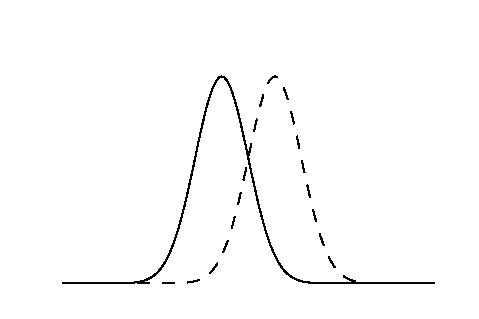
\includegraphics[height=1.5in]{figs/meanchange_lowvar}
\caption{ }
\end{subfigure}
~
\begin{subfigure}[b]{0.45\textwidth}
\centering
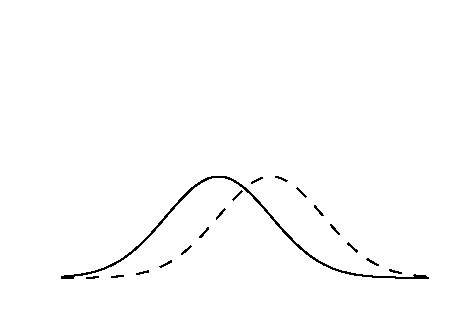
\includegraphics[height=1.5in]{figs/meanchange_highvar}
\caption{ }
\end{subfigure}
\caption{
 Changing the mean of a Gaussian by a fixed amount (from solid to
 dotted curve)
can have more impact
when the (shared) variance is small (as in a)
compared to when the variance is large (as in b).
Hence the impact (in terms of prediction accuracy)
of a change to $\mu$
depends on where the optimizer is in
$(\mu,\sigma)$ space.
\figtaken{Figure 3 of \citep{Honkela2010}, reproduced from 
\citep{ValpolaPhD}.}
\figthanks{Antti Honkela}.
}
\label{fig:honkelaGaussians}
\end{figure}

The key to NGD is to measure the notion of distance
between two probability distributions
in terms of the KL divergence.
This can be approximated in terms of
the \keywordDef{Fisher information matrix}  (FIM).
In particular, for any given input $\xdata$,
we have
\be
  \KLpq{p_{\params}(\vy|\xdata)}{p_{\params+\vdelta}(\vy|\xdata)}
  \approx
\half \vdelta^\trans \vFisher_{\xdata} \vdelta
\ee
where $\vFisher_{\xdata}$ is the FIM
\be
\vFisher_{\xdata}(\params)
= -\expectQ{\nabla^2 \log p_{\params}(\vy|\xdata)}{p_{\params}(\vy|\xdata)}
= \expectQ{(\nabla \log p_{\params}(\vy|\xdata))
(\nabla \log p_{\params}(\vy|\xdata))^\trans}{p_{\params}(\vy|\xdata)}
\ee
We  now replace the Euclidean distance
between the parameters,
$d(\vtheta_k, \vtheta_{k+1}) = ||\vdelta||_2^2$,
with 
\be
d(\vtheta_k, \vtheta_{k+1})
= \vdelta^\trans \vFisher_k \vdelta_k
\ee
where $\vdelta = \vtheta_{k+1}-\vtheta_k$
and $\vFisher_k = \vFisher_{\vx}(\vtheta_k)$
for a randomly chosen input $\vx$.
This gives rise to the following constrained
optimization problem:
\be
\vdelta_k = \argmin_{\vdelta}
\hat{\loss}_k(\vtheta_k + \vdelta) \myst
\vdelta^\trans \vFisher_k \vdelta \leq \epsilon
\ee
If we replace the constraint with a Lagrange multiplier,
we get the unconstrained objective:
\be
J_k(\vdelta) = \loss(\vtheta_k) + \vg_k^\trans \vdelta
+ \lr_k \vdelta^\trans \vFisher_k \vdelta 
\ee
Solving $J_k(\vdelta)=0$ gives the update
\be
\vdelta =  -\lr_k \vFisher_k^{-1} \vg_k
\ee
The term $\vFisher^{-1} \vg$
is called the \keywordDef{natural gradient}.
This is equivalent to  a preconditioned gradient update,
where we use the inverse FIM as a preconditioning matrix.
We can compute  the (adaptive) learning rate using
\be
\eta_k = \sqrt{\frac{\epsilon}{\vg_k^\trans \vF_k^{-1} \vg_k}}
\ee


Computing the FIM can be hard.
A simple approximation is to replace
the model's distribution with the empirical distribution.
In particular, define
 $\pemp(\xdata,\vy) = \frac{1}{N} \sum_{n=1}^N \delta_{\xdata_n}(\xdata) \delta_{\vy_n}(\vy)$,
$\pemp(\xdata) = \frac{1}{N} \sum_{n=1}^N \delta_{\xdata_n}(\xdata)$
and
$p_{\vtheta}(\vx,\vy) =  \pemp(\vx) p(\vy|\vx,\vtheta)$.
Then we can compute the \keywordDef{empirical Fisher}
\citep{Martens2016Thesis}
as follows:
\begin{align}
\vFisher(\vtheta) &= \expectQ{
\nabla \log p(\vy|\xdata,\params)
\nabla \log p(\vy|\xdata,\params)^\trans}
{p_{\vtheta}(\vx,\vy)} \\
 &\approx
\expectQ{
\nabla \log p(\vy|\xdata,\params)
\nabla \log p(\vy|\xdata,\params)^\trans}
{\pemp(\vx,\vy)} \\
&=
\frac{1}{|\data|}
\sum_{(\xdata,\vy) \in \data}
\nabla \log p(\vy|\xdata,\params)
\nabla \log p(\vy|\xdata,\params)^\trans
\end{align}

\subsubsection{Natural actor critic}

To apply NGD to RL, we can adapt
the A2C algorithm in \cref{algo:AC}.
In particular, define
\be
\vg_{kt} = \nabla_{\vtheta_k} A_t \log \pi_{\vtheta}(\va_t|\vs_t)
\ee
where $A_t$ is the advantage function at step $t$
of the random trajectory generated by the policy
at iteration  $k$.
Now we compute
\be
\vg_k = \frac{1}{T} \sum_{t=1}^T \vg_{kt},
\;
\vF_k = \frac{1}{T} \sum_{t=1}^T \vg_{kt} \vg_{kt}^\trans
\label{eqn:NACfisher}
\ee
and compute
$\vdelta_{k+1} = -\lr_k \vF_k^{-1} \vg_k$.
This approach is called \keywordDef{natural policy gradient}
\citep{Kakade2001,Rajeswaran2017}.

We can compute $\vF_k^{-1} \vg_k$ without having
to invert $\vF_k$ by using the conjugate gradient method,
where each CG step uses efficient
methods for Hessian-vector products \citep{Pearlmutter1994}.
This is called
\keywordDef{Hessian free optimization}  \citep{Martens2010}.
Similarly, we can efficiently compute
$\vg_k^\trans (\vF_{k}^{-1} \vg_k)$.

As a more accurate alternative
to the empirical Fisher,
\citep{Martens2015kfac} propose
the \keywordDef{KFAC} method,
which stands for ``Kronecker factored approximate curvature'';
this approximates the FIM of a DNN as a block diagonal
matrix, where each block is a Kronecker product
of two small matrices.
This was applied to policy gradient learning in \citep{Wu2017kfac}.


\eat{
\section{Bound optimization methods}

In this section, we describe methods that
aim to monotonically improve the performance of the policy
at each step,
similar to other \keywordDef{bound optimization} methods\footnote{
%
Bound optimization is also called \keywordDef{MM},
for majorize then maximize/minimize.
See \citep{Hunter04} for a tutorial.
} %
such as EM.
}

\section{Policy improvement methods}
\label{sec:polImprovement}
\label{sec:policyImprovement}

In this section, we discuss methods that try to monotonically
improve performance of the policy at each step,
rather than just following the gradient,
which can result in a high variance estimate
where performance can increase or decrease at each step.
These are called \keywordDef{policy improvement} methods.
Our presentation is based on \cite{Queeney2024}.

\subsection{Policy improvement lower bound}

We start by stating a useful result from
\citep{Achiam2017}.
Let $\pi_k$ be the current policy at step $k$,
and let $\pi$ be any other policy (e.g., a candidate new one).
Let  $\statdistpolk$ be the normalized
discounted state visitation distribution for $\policy_k$,
defined in \cref{eqn:statdistpol}.
Let $A^{\pi_k}(s,a) = Q^{\pi_k}(s,a)-V^{\pi_k}(s)$
be the advantage function.
Finally, let the total variation distance
between two distributions be
given by
\be
\text{TV}(p,q) \defeq \half ||\vp-\vq||_1
= \half \sum_s |p(s) - q(s)| 
\ee
Then one can show \citep{Achiam2017} that
\be
J(\pi) - J(\pi_k)
\geq
  \frac{1}{1-\gamma}
\underbrace{
 \expectQ{
  \frac{\pi(a|s)}{\pi_k(a|s)}
  A^{\pi_k}(s,a)}{\statdistpolk(s) \policy_k(a|s)}
}_{L(\pi,\pi_k)}
-
  \frac{2 \gamma C^{\pi,\pi_k}}{(1-\gamma)^2}
  \expectQ{\text{TV}(\pi(\cdot|s),\pi_k(\cdot|s))}{\statdistpolk(s)}
\label{eqn:Jlowerbound}
  \ee
where
$C^{\pi,\pi_k} = \max_s |\expectQ{A^{\pi_k}(s,a)}{\pi(a|s)}|$.
In the above, $L(\pi,\pi_k)$ is a  surrogate objective,
and the second term is a penalty term.

If we can optimize this lower bound (or a stochastic approximation,
based on samples from the current policy $\pi_k$),
we can guarantee monotonic policy improvement (in expectation)
at each step.
We will replace this objective with a trust-region update
that is easier to optimize:
\be
\pi_{k+1} = \argmax_{\pi} L(\pi,\pi_k)
\myst   \expectQ{\text{TV}(\pi,\pi_k)(s)}{\statdistpolk(s)} \leq
\epsilon
\label{eqn:polImprovementBound}
\ee
The constraint bounds the worst-case performance decline at each
update.
The overall procedure becomes an approximate policy improvement
method.
There are various ways of implementing the above method in practice,
some of which we discuss below.
(See also \citep{Grudzien2022}, who propose a framework
called \keywordDef{mirror learning},
that justifies these ``approximations'' as in fact being
the optimal thing to do for a different kind of objective.)



\subsection{Trust region policy optimization (TRPO)}
\label{sec:TRPO}



In this section, we describe
the \keywordDef{trust region policy optimization}
(\keywordDef{TRPO}) method of \citep{TRPO}.
This implements an approximation to \cref{eqn:polImprovementBound}.
First, it leverages the fact that if
\be
\expectQ{\KLpq{\pi_k}{\pi}(s)}{\statdistpolk(s)} \leq \delta
\ee
then $\pi$ also satisfies the TV constraint
with $\delta=\frac{\epsilon^2}{2}$.
Next it considers a first-order expansion of the surrogate objective
to get
\be
L(\pi,\pi_k)
=
 \expectQ{
  \frac{\pi(a|s)}{\pi_k(a|s)}
  A^{\pi_k}(s,a)}{\statdistpolk(s) \policy_k(a|s)}
\approx \vg_k^\trans (\vtheta-\vtheta_k)
\ee
where $\vg_k = \nabla_{\vtheta} L(\pi_{\vtheta},\pi_k)|_{\vtheta_k}$.
Finally it considers a second-order expansion of the KL term
to get the approximate constraint
\be
\expectQ{\KLpq{\pi_k}{\pi}(s)}{\statdistpolk(s)}
\approx \half (\vtheta-\vtheta_k)^\trans \vF_k (\vtheta-\vtheta_k)
\ee
where $\vF_k = \vg_k \vg_k^\trans$ is an approximation to
the Fisher information matrix
(see \cref{eqn:NACfisher}).
We then use the update
\be
\vtheta_{k+1} = \vtheta_k + \eta_k \vv_k
\ee
where $\vv_k = \vF_k^{-1} \vg_k$ is the natural gradient,
and the step size is initialized to
$\eta_k = \sqrt{\frac{2 \delta}{\vv_k^\trans \vF_k \vv_k}}$.
(In practice we compute $\vv_k$ by approximately
solving the linear system $\vF_k \vv = \vg_k$
using conjugate gradient methods,
which just require matrix vector multiplies.)
We then use a backtracking line search procedure
to ensure the trust region is satisfied.

\eat{
We start with a useful fact that relate
the policy values of two arbitrary policies
\citep{Kakade2002RL}:
\begin{align}
\polval(\policy')-\polval(\policy)
=  \expectQ{\expectQ{\Apol(s,a)}{\policy'(a|s)}}
{\statmeasure_{\policy'}(s)}
 \label{eqn:PolicySwitchThm}
\end{align}
where $\policy$ can be interpreted as the current policy during policy optimization, and $\policy'$ a candidate new policy (such as the greedy policy wrt $\Qpol$).
As in the policy improvement theorem
(\cref{sec:policyIteration}),
if $\expectQ{\Apol(s,a)}{\policy'(a|s)} \ge 0$ for all $s$,
then $\polval(\policy') \ge \polval(\policy)$.
However, we cannot ensure this condition to hold
when function approximation is used,
as such a uniformly improving policy $\policy'$
may not be representable by our parametric family.
Therefore, nonnegativity of \cref{eqn:PolicySwitchThm}
is not easy to ensure.


One way to ensure monotonic improvement of
$\polval$ is to improve the policy conservatively.
Let us define
\begin{align}
\polvallin( \policy')
 \defeq  \expectQ{\expectQ{\Apol(s,a)}{\policy'(a|s)}}{\statmeasure_{\policy}(s)}
 = \expectQ{\frac{\policy'(a|s)}{\policy(a|s)}
   \Apol(s,a)}{\statmeasure_{\policy}(s)\policy(a|s)}
 \label{eqn:polvalLin}
\end{align}
In the above,
we have switched the state distribution from
$\statmeasure_{\policy'}$ in \cref{eqn:PolicySwitchThm}
to $\statmeasure_{\policy}$.
In \citep{TRPO} they show that
we have  we have the following lower bound on the improvement:
\be
J(\pi') - J(\pi) \geq L(\pi') - C \max_s \KLpq{\pi(a|s)}{\pi'(a|s)}
\label{eqn:JlowerBound}
\ee
where $C$  is a constant.
We can approximate the max over states with an expectation,
to get the  following constrained optimization problem:
\begin{align}
\label{eqn:TRPOconstr}
\argmax_{\policy'}
 \polvallin(\policy')
 \myst
 \expectQ{\KLpq{\policy(\cdot|s)}{\policy'(\cdot|s)}}
         {\statmeasure_{\policy}(s)} \leq \delta
\end{align}
for some threshold $\delta>0$.
We can then approximate the KL term with the Fisher information
matrix, as in \cref{sec:NGD}.
This gives the update
\be
\vtheta_{k+1} = \vtheta_k + \lr_k \vF(\vtheta_k)^{-1}
  \nabla_{\vtheta} L(\vtheta)\vert_{\vtheta_k}
  \ee
 We  can compute $\lr_k$ using a linesearch procedure:
 we start with largest value for $\lr_k$ allowed by the KL constraint,
 and reduce it until
 the lower bound is positive.
}


\subsection{Proximal Policy Optimization (PPO)}
\label{sec:PPO}

In this section, we describe the
the \keywordDef{proximal policy optimization}
or \keywordDef{PPO} method of \citep{PPO},
which is a simplification of TRPO.
%Note that PPO does not guarantee monotonic improvement,
%but can be modified to do so
%\citep{Wang2019PPO}.
%The blog post at \url{https://vitalab.github.io/article/2020/01/14/Implementation\_Matters.html}
%argues that the benefits of PPO over TRPO follow more from
%code-level optimizations than the objective itself.
%See  \url{https://iclr-blog-track.github.io/2022/03/25/ppo-implementation-details/}


We start by noting the following result:
\be
\expectQ{\text{TV}(\pi,\pi_k)(s)}{\statdistpolk(s)}
= \half \expectQ{| \frac{\pi(a|s)}{\pi_k(a|s)} - 1 |}
{(s,a) \sim \statdistpolk}
\ee
This holds provided the support of $\pi$ is contained
in the support of $\pi_k$ at every state.
We then use the following update:
\be
\pi_{k+1} = \argmax_{\pi} 
\expectQ{
  \min\left( \rho_k(s,a)  A^{\pi_k}(s,a),
  \tilde{\rho}_k(s,a)  A^{\pi_k}(s,a)
  \right)}{(s,a) \sim \statdistpolk}
\ee
where $\rho_k(s,a) = \frac{\pi(a|s)}{\pi_k(a|s)}$
is the likelihood ratio, and
$\tilde{\rho}_k(s,a)= \text{clip}(\rho_k(s,a), 1-\epsilon,
1+\epsilon)$,
where $\text{clip}(x,l,u) = \min(\max(x,l),u)$.
\eat{
We start by considering the following unconstrained objective,
based on \cref{eqn:JlowerBound}:
\begin{align}
  \polval(\policy') = \polvallin(\policy')
  - \beta\expectQ{\KLpq{\policy(\cdot|s)}{\policy'(\cdot|s)}}
  {\statmeasure_{\policy}(s)}
\end{align}
where
\begin{align}
\polvallin( \policy')
 = \expectQ{\frac{\policy'(a|s)}{\policy(a|s)}
   \Apol(s,a)}{\statmeasure_{\policy}(s)\policy(a|s)}
\end{align}
Unfortunately, the likelihood ratio
\be
l(s,a) = \frac{\pi'(a|s)}{\pi(a|s)}
\ee
which is needed to compute $\polvallin(\policy')$
might become very large or small, if $\pi'$ deviates too much
from $\pi$. To ensure stability we can replace it with
\be
\tilde{l}(s,a) = 
\text{clip}(r(s,a;\vtheta), 1-\epsilon, 1+\epsilon)
\ee
which ensures $|l(s,a;\vtheta) - 1| \leq \epsilon$.
Furthermore, we can drop the KL penalty and just optimize
\be
\polval(\vtheta) = \expect{\min(l(s,a;\vtheta) \Apol(s,a), \;\;
\tilde{l}(s,a;\vtheta) \Apol(s,a))}
\ee
}
See \citep{Grudzien2022} for a theoretical justification
for these simplifications.
Furthermore,
this can be modified to ensure monotonic
improvement as discussed in \citep{Wang2019PPO},
making it a true bound optimization method.


Some pseudocode for PPO (with GAE)
is given in \cref{algo:PPO}.
It is basically identical to the AC code in \cref{algo:AC},
except the policy loss has the form
$\min(\rho_t A_t, \tilde{\rho}_t A_t)$
instead of
$A_t \log \pi_{\vphi}(a_t|s_t)$,
and we perform multiple policy updates per rollout,
for increased sample efficiency.
For all the implementation details, see
\url{https://iclr-blog-track.github.io/2022/03/25/ppo-implementation-details/}.


\begin{algorithm}
\dontprintsemicolon
\caption{PPO  with GAE}
\label{algo:PPO}
Initialize  parameters $\vphi$, 
environment state $s$\\
\For{iteration $k=1,2,\ldots$}
{
  $(\tau,s) = \text{rollout}(s, \pi_{\vphi})$ \\
  $(s_1,a_1,r_1,\ldots,s_T)= \tau$ \\
  $v_{t} = V_{\vphi}(s_{t}) \; \text{for } t=1:T$ \\
  $(A_{1:T}, \targetV_{1:T}) = \text{GAE}(r_{1:T}, v_{1:T}, \gamma, \lambda)$
  \\
  $\vphi_{\old} \assign \vphi$ \\
  \For{$m=1:M$}{
  $\rho_{t} = \frac{\pi_{\vphi}(a_t|s_t)}{\pi_{\vphi_{\old}}(a_t|s_t)}
  \; \text{for } t=1:T$  \\
  $\tilde{\rho}_t = \text{clip}(\rho_t) \text{ for } t=1:T$ \\
  $\loss(\vphi) = \frac{1}{T}\sum_{t=1}^T \left[
    \lambda_{TD} (V_{\vphi}(s_t) - \targetV_t)^2
    -\lambda_{PG} \min(\rho_t A_t, \tilde{\rho}_t A_t)
    -\lambda_{ent} \entropy(\pi_{\vphi}(\cdot|s_t)) \right]$ \\
  $\vphi := \vphi -  \lr \nabla_{\vphi} \loss(\vphi)$ \\
  }
}
\end{algorithm}


\eat{
\begin{algorithm}
\dontprintsemicolon
\caption{PPO with $1$-step critic}
\label{algo:PPO}
Initializeparameters $\vphi$,
environment state $s$\\
\Repeat{converged}
{
  $(\tau,s) = \text{rollout}(s, \pi_{\vtheta})$ \\
  \For{$k=1:K$}{
    $\vphi_{\old}=\vphi$ \\
    $\vphi = \text{PPO-step}(\tau, \vphi,  \vphi_{\old})$ \\
    }
}
.\\
$\text{def PPO-step}(\tau, \vphi, \vphi_{\old})$: \\
Let $(s_0,a_0,r_0,\ldots,s_T)=\tau$ \\
\For{$t=0:T-1$}{
  $G_t = r_{t+1} + \gamma V_{\vphi}(s_{t+1})$ \\
  $A_t = \stopgrad(G_t - V_{\vphi}(s_t))$ \\
  $r_t = \frac{\pi_{\vphi}(a_t|s_t)}{\pi_{\vphi_{\old}}(a_t|s_t)}$
  \\
  $\tilde{r}_t = \text{clip}(r_t)$ \\
}
$\loss = \frac{1}{T} \sum_t \left[
  \lambda_V (V_{\vphi}(s_t) - G_t)^2
  -\lambda_{\pi} \min(r_t A_t, \tilde{r}_t A_t)
  -\lambda_{ent} \entropy(\pi_{\vphi}(\cdot|s_t)) \right]$ \\
$\vphi \assign \vphi - \lr \nabla \loss$\\
       Return $\vphi$
\end{algorithm}
}

% https://github.com/luchris429/purejaxrl/blob/main/purejaxrl/ppo.py#L173
% https://github.com/snu-mllab/Achievement-Distillation/blob/main/achievement_distillation/model/ppo.py#L107

\eat{
\begin{algorithm}
\dontprintsemicolon
\caption{PPO with $1$-step critic}
\label{algo:PPO}
Initialize actor parameters $\vtheta$, critic parameters $\vw$,
environment state $s$\\
\Repeat{converged}
{
  $(\tau,s) = \text{rollout}(s, \pi_{\vtheta})$ \\
  \For{$k=1:K$}{
    $\vtheta_{\old}=\vtheta$ \\
    $(\vtheta, \vw) = \text{PPO-step}(\vtheta, \vw, \tau, \vtheta_{\old})$ \\
    }
}
.\\
$\text{def PPO-step}(\vtheta,\vw,\tau,\vtheta_{\old})$: \\
Let $(s_0,a_0,r_0,\ldots,s_T)=\tau$ \\
\For{$t=0:T-1$}{
  $Q_t = r_{t+1} + \gamma V_{\vw}(s_{t+1})$ \\
  $A_t = \stopgrad(Q_t - V_{\vw}(s_t))$ \\
  $r_t = \frac{\pi_{\vtheta}(a_t|s_t)}{\pi_{\vtheta_{\old}}(a_t|s_t)}$
  \\
  $\tilde{r}_t = \text{clip}(r_t)$ \\
}
$\loss_{\vw} = \frac{1}{T} \sum_t (V_{\vw}(s_t) - \stopgrad(Q_t))^2$ \\
$\loss_{\vtheta} = -\frac{1}{T} \sum_t 
\min(r_t A_t, \tilde{r}_t A_t)$ \\
$\vw \assign \vw - \lr_{\vw} \nabla \loss_{\vw}$\\
$\vtheta \assign \vtheta - \lr_{\vtheta} \nabla \loss_{\vtheta}$ \\
       Return $(\vtheta,\vw)$
\end{algorithm}
}



\subsection{VMPO}
\label{sec:MPO}
\label{sec:VMPO}


In this section, we discuss
the \keywordDef{VMPO} algorithm of \citep{VMPO},
which is an on-policy extenson of the earlier
on-policy \keywordDef{MPO} algorithm (MAP policy optimization)
from \citep{Abdolmaleki2018}.
It was originally explained in terms of ``control as inference''
(see \cref{sec:inferRL}),
but we can also view it as
a  contrained policy improvement method,
based on   \cref{eqn:polImprovementBound}.
In particular, VMPO leverages the fact that if
\be
\expectQ{\KLpq{\pi}{\pi_k}(s)}{\statdistpolk(s)} \leq \delta
\ee
then $\pi$ also satisfies the TV constraint
with $\delta=\frac{\epsilon^2}{2}$.

Note that here the KL is reversed compared to TRPO
in \cref{sec:TRPO}.
This new version will encourage $\pi$
to be mode-covering, so it will naturally
have high entropy, which can result in improved robustness.
Unfortunately, this kind of KL is harder to compute,
since we are taking expectations wrt the unknown distribution $\pi$.

To solve this problem, VMPO adopts an EM-type approach.
In the E step, we compute a non-parametric version
of the state-action distribution given by the unknown
new policy:
\be
\psi(s,a) = \pi(a|s) \statdistpolk(s)
\ee
The optimal new distribution is given by
\be
\psi_{k+1} = \argmax_{\psi}
\expectQ{A^{\pi_k}(s,a)}{\psi(s,a)}
\myst \KLpq{\psi}{\psi_k} \leq \delta
\ee
where
$\psi_k(s,a) = \pi_k(a|s) \statdistpolk(s)$.
The solution to this  is
\begin{align}
  \psi_{k+1}(s,a) &=  \statdistpolk(s) \pi_k(a|s) w(s,a) \\
  w(s,a) &= \frac{\exp(A^{\pi_k}(s,a)/\lambda^*)}{Z(\lambda^*)} \\
  Z(\lambda) &= \expectQ{\exp(A^{\pi_k}(s,a)/\lambda)}{(s,a)\sim
    \statdistpolk} \\
  \lambda^* &= \argmin_{\lambda \geq 0} \lambda \delta + \lambda \log Z(\lambda)
  \end{align}
In the M step, we project this target distribution back onto the space
of parametric policies, while satisfying the KL trust region
constraint:
\be
\pi_{k+1} = \argmax_{\pi}
\expectQ{w(s,a) \log \pi(a|s)}{(s,a) \sim \statdistpolk}
\myst \expectQ{\KLpq{\psi_k}{\psi}(s)}{\statdistpolk} \leq \delta
\ee


\section{Off-policy methods}
\label{sec:offPolicy}
\label{sec:offpolicy}


In many cases, it is useful to train a policy
using data collected from a distinct
\keywordDef{behavior policy}
$\behavior(a|s)$ that is
not the same as the \keywordDef{target policy} $\policytgt(a|s)$
that is being learned.
For example, this could be data collected
from earlier trials or parallel workers
(with different parameters $\vtheta'$)
and stored in a \keywordDef{replay buffer},
or it could be \keywordDef{demonstration data} from human experts.
This is known as \keywordDef{off-policy RL},
and can be much more sample efficient than the on-policy 
methods we have discussed so far, since these methods
can use data from multiple sources.
However, off-policy methods are more complicated,
as we will explain below.

The basic difficulty  is that the target policy  that we want to learn
may want to try an action in a state that has
not been experienced before in the existing data,
so there is no way to predict the outcome of this new $(s,a)$
pair.
In this section, we tackle this problem by assuming
that the  target policy is not too different from the behavior policy,
so that the ratio $\policytgt(a|s)/\policybeh(a|s)$
is bounded, which allows us to use methods based on importance
sampling.
%(In particular, this means that the behavior
%policy must have broad enough support that it covers the target.)
In the online learning setting, we can ensure this property
by using conservative incremental updates to the policy.
%as we discuss in \cref{sec:offpolPolImprovement}.
Alternatively we can use policy gradient methods
with various regularization methods, as we discuss below.

In \cref{sec:offlineRL}, we discuss offline RL,
which is an extreme instance of off-policy RL where we
have a fixed behavioral dataset, possibly generated from an unknown
behavior policy,
and can never collect any new data.



\subsection{Policy evaluation using importance sampling}
\label{sec:offpolicyRL-IS}

Assume we have a dataset of the form
$\data = \{\traj^{(i)}\}_{1 \le i \le n}$, where each trajectory is a sequence
$\traj^{(i)}=(s_0^{(i)},a_0^{(i)},r_0^{(i)},s_1^{(i)}\ldots)$,
where the actions are sampled according to a behavior policy
$\policybeh$, and
the reward and next states are sampled
according to the reward and transition models.
We want to use this offline dataset to evaluate the performance of some
target policy $\policytgt$;
this is called \keywordDef{off-policy policy evaluation} or \keywordDef{OPE}.
If the trajectories $\traj^{(i)}$ were sampled from $\policytgt$.
we could use the standard Monte Carlo estimate:
\begin{align}
  \hat{J}(\policytgt)
\defeq \frac{1}{n} \sum_{i=1}^n  \sum_{t=0}^{T-1} \gamma^t r_t^{(i)}
\end{align}
However, since the trajectories are sampled from $\policybeh$,
we use \keywordDef{importance sampling} (IS)
to correct for the distributional mismatch,
as first proposed in \citep{Precup2000}.
This gives
\begin{align}
\label{eqn:offpolicyrl-basicis}
  \polvalis(\policytgt)
  \defeq \frac{1}{n} \sum_{i=1}^n
  \frac{p(\traj^{(i)}|\policytgt)}{p(\traj^{(i)}|\policybeh)}
  \sum_{t=0}^{T-1} \gamma^t r_t^{(i)}
\end{align}
It can be verified that $\expectQ{\polvalis(\policytgt)}{\policybeh}
= \polval(\policytgt)$, that is, $\polvalis(\policytgt)$ is \keywordDef{unbiased},
provided that $p(\traj|\policybeh)>0$
whenever $p(\traj|\policytgt)>0$.
The \keywordDef{importance ratio},
$\frac{p(\traj^{(i)}|\policytgt)}{p(\traj^{(i)}|\policybeh)}$,
is used to compensate for the fact that
the data is sampled from $\policybeh$ and not $\policytgt$.
It can be simplified as follows:
\begin{align}
\label{eqn:offpolicyrl-isratio}
\frac{p(\traj|\policytgt)}{p(\traj|\policybeh)}
= \frac{p(s_0) \prod_{t=0}^{T-1} \policytgt(a_t|s_t) \ptran(s_{t+1}|s_t,a_t) \preward(r_t|s_t,a_t,s_{t+1})}{p(s_0) \prod_{t=0}^{T-1} \policybeh(a_t|s_t) \ptran(s_{t+1}|s_t,a_t) \preward(r_t|s_t,a_t,s_{t+1})}
= \prod_{t=0}^{T-1} \frac{\policytgt(a_t|s_t)}{\policybeh(a_t|s_t)}
\end{align}
This simplification makes it easy to apply IS,
as long as the target and behavior policies are known.
(If the behavior policy is unknown,
we can estimate it from $\data$,  and replace $\policybeh$
by its estimate $\hat{\policybeh}$.
For convenience, define the
\keywordDef{per-step importance ratio} at time $t$ by
\be
\psiRatio_t(\traj) \defeq \policytgt(a_t|s_t) / \policybeh(a_t|s_t)
\ee
We can reduce the variance of the estimator
by noting that the reward $r_t$ is independent of the trajectory
beyond time $t$.
This leads to a \keywordDef{per-decision importance sampling} variant:
\begin{align}
\label{eqn:offpolicyrl-pdis}
  \polvalpdis(\policytgt)
  \defeq \frac{1}{n} \sum_{i=1}^n \sum_{t=0}^{T-1}
  \prod_{t' \le t} \psiRatio_{t'}(\traj^{(i)}) \gamma^t r_t^{(i)}
\end{align}

\subsection{Off-policy actor critic methods}
\label{sec:offPolicyPG}

In this section, we discuss how to extend actor-critic
methods to work with off-policy data.

\subsubsection{Learning the critic using V-trace}
\label{sec:Vtrace}

In this section
we build on \cref{sec:offpolicyRL-IS} to develop a practical method,
known as \keywordDef{V-trace} \citep{Espeholt2018},
to estimate the value function for a target policy
using off-policy data.
(This is an extension of the earlier
\keywordDef{Retrace} algorithm \citep{Munos16},
which estimates the $Q$ function using off-policy data.)

First consider the $n$-step target value for $V(s_i)$
in the on-policy case:
\begin{align}
  V_i  &= V(s_i)
  + \sum_{t=i}^{i+n-1} \gamma^{t-i} r_t + \gamma^n V(s_{i+n}) \\
  &= V(s_i)
  + \sum_{t=i}^{i+n-1} \gamma^{t-i}
  \underbrace{(r_t + \gamma V(s_{t+1}) - V(s_t))}_{\delta_t}
\end{align}
where we define $\delta_t  = (r_t + \gamma V(s_{t+1}) - V(s_t))$
as the TD error at time $t$.
To extend this to the off-policy case, we use the per-step
importance ratio trick. However, to bound the variance
of the estimator, we truncate the IS weights.
In particular, we define
\begin{align}
  c_t &= \min\left(\overline{c},
  \frac{\policytgt(a_t|s_t)}{\policybeh(a_t|s_t)} \right),
  \;
  \rho_t = \min\left(\overline{\rho},
  \frac{\policytgt(a_t|s_t)}{\policybeh(a_t|s_t)} \right) 
\end{align}
where $\overline{c}$ and $\overline{\rho}$
are hyperparameters.
We then define the V-trace target value for $V(s_i)$ as
\begin{align}
  v_i
  &= V(s_i)
  + \sum_{t=i}^{i+n-1} \gamma^{t-i} \left( \prod_{t'=i}^{t-1} c_{t'}
  \right)   \rho_t \delta_t
\end{align}
Note that we can compute these targets recursively using
\be
v_i = V(s_i) + \rho_i  \delta_i + \gamma c_i (v_{i+1} - V(s_{i+1}))
\ee

The product of the weights $c_i \ldots c_{t-1}$ (known as the ``trace'')
measures how much a temporal difference $\delta_t$
at time $t$ impacts the update of the value function
at earlier time $i$.
If the policies are very different, the variance of this product
will be large. So the truncation parameter $\overline{c}$
is used to reduce the variance.
In  \citep{Espeholt2018}, they find $\overline{c}=1$ works best.

The use of the target $\rho_t \delta_t$  rather than $\delta_t$
means we are evaluating the value function for a policy
that is somewhere between $\policybeh$ and $\policytgt$.
For $\overline{\rho}=\infty$ (i.e., no truncation),
we converge to the value function $V^{\policytgt}$,
and for $\overline{\rho} \ra 0$,
we converge to the value function $V^{\policybeh}$.
In  \citep{Espeholt2018}, they find $\overline{\rho}=1$ works best.

Note that if $\overline{c}=\overline{\rho}$,
then $c_i=\rho_i$. This gives rise to the simplified form
\begin{align}
  v_t
  &= V(s_t)
  + \sum_{j=0}^{n-1} \gamma^{j} \left( \prod_{m=0}^{j} c_{t+m}
  \right)   \delta_{t+j}
  \label{eqn:Vtrace}
\end{align}

We can use the above V-trace targets to learn an approximate
value function by minimizing the usual $\ell_2$ loss:
\be
\loss(\vw) = \expectQ{(v_t - V_{\vw}(s_t))^2}{t \sim \data}
\ee
the gradient of which has the form
\be
\nabla \loss(\vw) = 2 \expectQ{(v_t - V_{\vw}(s_t))
  \nabla_{\vw}  V_{\vw}(s_t)}{t \sim \data}
\ee


\subsubsection{Learning the actor}
\label{sec:offpolPG}

We now discuss how to update the actor
using an off-policy estimate of the policy gradient.
We start by defining the objective to be
the expected value of the new policy,
where the states are drawn from the behavior
policy's state distribution, but the actions
are drawn from the target policy:
\be
J_{\behavior}(\policy_{\vtheta})
= \sum_s \statdistbehave(s) \Vpol(s)
= \sum_s \statdistbehave(s) \sum_a \policy_{\vtheta}(a|s) \Qpol(s,a)
\label{eqn:offPolicyJ}
\ee
Differentiating this and
ignoring the term $\nabla_{\vtheta} \Qpol(s,a)$, as suggested by \citep{Degris2012},
gives a way to (approximately) estimate the
\keywordDef{off-policy policy-gradient}
using a one-step IS correction ratio:
\begin{align}
\nabla_{\vtheta}
 J_{\behavior}(\policy_{\vtheta})
  &\approx \sum_s \sum_a
  \statdistbehave(s) \nabla_{\vtheta} \policy_{\vtheta}(a|s) \Qpol(s,a) \\
  &= \expectQ{  \frac{\policy_{\vtheta}(a|s)}{\behavior(a|s)}
  \nabla_{\vtheta} \log \policy_{\vtheta}(a|s) \Qpol(s,a)}
  {\statdistbehave(s), \behavior(a|s)}
\end{align}

In practice, we can approximate $Q_{\pi}(s_t,a_t)$
by $q_t = r_t + \gamma v_{t+1}$,
where $v_{t+1}$ is the V-trace estimate for state $s_{t+1}$.
If we use $V(s_t)$ as a baseline, to reduce the variance,
we get the following gradient estimate for the policy:
\be
\nabla J(\vtheta) = \expectQ{
  \rho_t \nabla_{\vtheta} \log \pi_{\vtheta}(a_t|s_t)
  (r_t + \gamma v_t - V_{\vw}(s_t))}{t \sim \data}
\ee

We can also replace the 1-step IS-weighted TD error
$\rho_t (r_t + \gamma v_t - V_{\vw}(s_t))$
with an IS-weighted GAE value
by modifying the generalized advantage estimation method
in \cref{sec:GAE}.
In particular, we just need to define
$\lambda_t = \lambda \min(1, \rho_t)$.
We denote the IS-weighted GAE estimate  as $A_t^{\rho}$.\footnote{
  %
  For an implementation, see
  \url{https://github.com/google-deepmind/rlax/blob/master/rlax/\_src/multistep.py\#L39}
  }

\subsubsection{IMPALA}
\label{sec:IMPALA}

As an example of an off-policy AC method,
we consider
\keywordDef{IMPALA},
which stands for ``Importance Weighted Actor-Learning Architecture''.
\citep{Espeholt2018}.
This uses  shared parameters for the policy and value function
(with different output heads), and adds an entropy bonus
to ensure the policy remains stochastic.
Thus we end up with the following objective,
which is very similar to on-policy actor-critic
shown in \cref{algo:AC}:
\be
  \loss(\vphi) = \expectQ{
    \lambda_{TD} (V_{\vphi}(s_t) - v_t)^2
    -\lambda_{PG} A_t^{\rho} \log \pi_{\vphi}(a_t|s_t)
    -\lambda_{ent} \entropy(\pi_{\vphi}(\cdot|s_t))
  }{t \sim \data}
  \label{eqn:offpolAC}
  \ee
The only difference from standard A2C is that we need
to store the probabilities of each action,
$\policybeh(a_t|s_t)$, in addition to $(s_t,a_t,r_t,s_{t+1})$
in the dataset $\data$,
which can be used to compute $\rho_t$.
\citep{Espeholt2018} was  able to use this method to train 
a single agent (using a shared CNN and LSTM for both value and policy)
to play all 57 games at a high level.
Furthermore, they showed that their
method --- thanks to its off-policy corrections ---
outperformed the A3C method (a parallel version of A2C) in \cref{sec:A3C}.



 \eat{
The term $\frac{\policy_{\vtheta}(a|s)}{\behavior(a|s)}$
is an \keywordDef{importance sampling} correction term,
used to compensate for the fact that the data is sampled
from $\behavior$ and not $\policy$.
We require that  the support of the behavior
policy  is at least
as broad as the target policy,
so $\policy(a|s)>0 \implies \behavior(a|s)>0$.
Also,  to ensure the variance of the estimators is reasonable,
we require that $\behavior$ be close to $\policy$.
This can be problematic in cases where the behavioral
data is log data that is created offline by some other system.
See \cref{sec:offlineRL} for a discussion of such cases.
In online RL, we can ensure the new policy does not
differ too much from the old policy, using methods
such as TRPO (\cref{sec:TRPO}),
PPO (\cref{sec:PPO}) and MPO (\cref{sec:MPO}).
In  \cref{sec:DPG},
we discuss a way to avoid the need to compute the IS ratio.
}





\subsection{Off-policy policy improvement methods}
\label{sec:offpolPolImprovement}

So far we have focused on  actor-critic methods.
However, policy improvement methods, such as PPO,
are often preferred to AC methods,
since they monotonically improve the objective.
In  \citep{Queeney2021} they propose
one way to extend PPO to the off-policy case.
This method was generalized in  \cite{Queeney2024}
to cover a variety of policy improvement algorithms,
including TRPO and VMPO.
We give a brief summary below.

The key insight is to realize that we can generalize
the lower bound in \cref{eqn:Jlowerbound}
to any reference policy 
\be
J(\pi) - J(\pi_k)
\geq
  \frac{1}{1-\gamma}
 \expectQ{
  \frac{\pi(a|s)}{\policyref(a|s)}
  A^{\pi_k}(s,a)}{\statdistpolref(s) \policy_k(a|s)}
-
  \frac{2 \gamma C^{\pi,\pi_k}}{(1-\gamma)^2}
  \expectQ{\text{TV}(\pi(\cdot|s),\policyref(\cdot|s))}{\statdistpolref(s)}
  \ee
The reference policy can be any previous policy,
or a convex combination of them.
In particular, if $\pi_k$ is the current policy,
we can consider the reference policy to be
$\policyref = \sum_{i=1}^M \nu_i \pi_{k-i}$,
where $0 \leq \nu_i \leq 1$
and $\sum_i \nu_i = 1$ are mixture weights.
We can approximate the expectation
by sampling  from the  replay buffer,
which contains samples from older policies.
That is, $(s,a) \sim \statdistpolref$
can be implemented by $i \sim \nu$
and $(s,a) \sim \statdistpolki$.

To compute the advantage function $A^{\pi_k}$
from off policy data, we can adapt the V-trace
method of \cref{eqn:Vtrace} to get
\begin{align}
  A_{\ttrace}^{\pi_k}(s_t,a_t)
  &= \delta_t
  + \sum_{j=0}^{n-1} \gamma^{j} \left( \prod_{m=1}^{j} c_{t+m}
  \right)   \delta_{t+j}
\end{align}
where
$\delta_t = r_t + \gamma V(s_{t+1}) - V(s_t)$,
and
$c_t = \min\left(\overline{c},
\frac{\pi_k(a_t|s_t)}{\pi_{k-i}(a_t|s_t)} \right)$
is the truncated importance sampling ratio.


To compute the TV penalty term from off policy data,
we need to choose between the PPO (\cref{sec:PPO}),
VMPO (\cref{sec:VMPO})
and TRPO (\cref{sec:TRPO}) approach.
We discuss each of these cases below.

\subsubsection{Off-policy PPO}

The simplest is to use off-policy PPO, which gives an update of the
following form (known as \keywordDef{Generalized PPO}):
\be
\pi_{k+1} = \argmax_{\pi} \expectQ{
  \expectQ{
    \min( \rho_{k-i}(s,a) A^{\pi_k}(s,a),
    \tilde{\rho}_{k-i}(s,a) A^{\pi_k}(s,a) )
  }{(s,a) \sim \statdistpolki}
  }{i \sim \nu}
\ee
where $\rho_{k-i}(s,a)=\frac{\pi(a|s)}{\pi_{k-i}(a|s)}$
and
$\tilde{\rho}_{k-i}(s,a)=\text{clip}(\frac{\pi(a|s)}{\pi_{k-i}(a|s)},l,u)$,
where $l=\frac{\pi_k(a|s)}{\pi_{k-i}(a|s)} - \epsilon$
and $u=\frac{\pi_k(a|s)}{\pi_{k-i}(a|s)} + \epsilon$.
(For other off-policy variants of PPO,
see e.g., \citep{Meng2023,Li2024R3}.)

\subsubsection{Off-policy VMPO}

%For details on the off-policy version of TRPO,
%please see \cite{Queeney2024}.
For an off-policy version of VMPO,
see  the original \keywordDef{MPO} method of \citep{Abdolmaleki2018};
this is derived using an EM framework,
but EM is just another bound optimization algorithm \citep{Hunter04},
and the result is equivalent to the version presented
in \cite{Queeney2024}.

\subsubsection{Off-policy TRPO}

For details on the off-policy version of TRPO,
see  \cite{Queeney2024}.


\subsection{Soft actor-critic (SAC)}
\label{sec:SAC}

\eat{
  https://chatgpt.com/c/6738ba70-9e20-8005-8092-2f516bd35d24
  
  
  Soft Actor-Critic (SAC) is an off-policy reinforcement learning algorithm that avoids the need for importance sampling through its unique design involving entropy maximization and how it structures its policy updates.

### Key Reasons SAC Avoids Importance Sampling:

1. **Policy and Q-Function Design**:
   SAC employs a stochastic actor-critic framework where the policy (actor) is updated using the reparameterization trick, which bypasses the need for importance sampling weights. The reparameterization trick allows gradients to be estimated directly by differentiating through the sampling process. This ensures that updates to the policy do not require the computation of density ratios that are typical in algorithms using importance sampling.

2. **Entropy Maximization**:
   SAC incorporates an entropy term in its objective function, encouraging exploration by maximizing the entropy of the policy. This approach smooths the policy update process and reduces the variance of the gradient estimates, leading to more stable training without needing importance sampling. By doing so, the policy learns to balance between maximizing the expected return and maintaining stochasticity, allowing it to sample actions effectively from a broad distribution.

3. **Off-Policy Learning with Replay Buffer**:
   Although SAC is off-policy and utilizes a replay buffer to sample past experiences, the policy update is done using the actor's own probability distribution, eliminating the need to correct for discrepancies between the behavior policy (used to collect data) and the target policy (used for updating). This means SAC directly optimizes the policy without needing to adjust for how likely each action was under the policy that generated it, thus avoiding importance sampling weights.

4. **Q-Value Estimation**:
   SAC uses a soft value function that incorporates the entropy of the policy, which implicitly handles any potential bias introduced by the use of past experiences. This soft value helps regularize the policy updates and ensures that the algorithm can handle off-policy data smoothly without additional corrections typically needed in importance sampling.

   In summary, SAC's combination of entropy maximization, the reparameterization trick for policy updates, and its clever handling of the value function enables it to perform off-policy learning while avoiding the complexity and potential variance associated with importance sampling.
}

\eat{
  Yes, the Maximum a Posteriori Policy Optimization (MPO) algorithm, being an off-policy algorithm, does involve importance sampling, but it uses it in a way that minimizes its typical downsides, such as high variance. Here's how MPO integrates importance sampling and manages it effectively:

### Importance Sampling in MPO:

1. **Policy Update**:
   MPO performs policy updates using a two-step approach:
   - **E-Step (Expectation Step)**: The algorithm computes the expected return under the current policy by sampling from a replay buffer. During this step, importance sampling weights are used to correct for the difference between the behavior policy (the policy that generated the data) and the target policy (the policy being optimized).
   - **M-Step (Maximization Step)**: MPO then fits a new policy to the distribution of actions obtained from the E-step by minimizing a Kullback–Leibler (KL) divergence between the target action distribution and the policy.

2. **Managing Importance Sampling Weights**:
   - To mitigate the high variance often associated with importance sampling, MPO employs a **clipping** technique. This limits the magnitude of the importance sampling weights, ensuring that overly large weights do not destabilize the learning process.
   - The algorithm carefully chooses the behavior policy to maintain overlap with the target policy. By ensuring that the data in the replay buffer is relevant to the current policy, MPO can reduce the variance of the importance weights.

3. **Regularization Through KL Constraints**:
   - MPO uses a KL constraint to limit how much the new policy can deviate from the current policy. This helps control the change in policy distribution, making the policy update more stable and reducing the variance introduced by importance sampling.
   - By fitting a parametric policy to the non-parametric distribution obtained during the E-step, MPO can leverage the advantages of importance sampling while keeping the updates reliable and controlled.

### Summary:
   While MPO does require importance sampling as part of its policy update process, it incorporates mechanisms such as clipping and KL constraints to mitigate the typical issues related to high variance and instability. This approach allows MPO to balance the use of off-policy data effectively, enabling robust learning without the negative effects that pure, unregulated importance sampling can bring.
}

\eat{

  Determining whether Soft Actor-Critic (SAC) or Maximum a Posteriori Policy Optimization (MPO) is better for off-policy reinforcement learning depends on the specific context, application, and requirements of the task at hand. Both algorithms have their strengths and trade-offs:

### Strengths and Considerations for SAC:
1. **Stability and Robustness**:
   - SAC is known for its stability due to its entropy-regularized objective function, which encourages exploration by maximizing policy entropy. This leads to robust learning, especially in environments where exploring various actions is beneficial.
2. **Ease of Implementation**:
   - SAC is relatively straightforward to implement and has been shown to perform well across a variety of continuous control tasks with minimal tuning.
3. **Entropy Maximization**:
   - The entropy term helps the policy remain stochastic, allowing SAC to explore effectively and avoid getting stuck in suboptimal deterministic policies.
4. **No Importance Sampling**:
   - SAC does not require importance sampling, which simplifies its implementation and avoids potential issues with high variance corrections common in off-policy algorithms that use importance sampling.

### Strengths and Considerations for MPO:
1. **Sample Efficiency**:
   - MPO has been designed to balance exploration and exploitation effectively by using a trust region approach to constrain policy updates. This can make MPO more sample-efficient than SAC in certain environments.
2. **Structured Policy Updates**:
   - MPO’s two-step process (E-step and M-step) ensures that the policy is updated in a controlled manner using KL constraints, which helps maintain stability.
3. **Adaptability to Different Objectives**:
   - MPO can be adapted to different reward structures and objectives by adjusting the weighting of the KL divergence term and other hyperparameters.
4. **Importance Sampling with Regularization**:
   - While MPO uses importance sampling for off-policy corrections, it mitigates high variance with techniques like clipping and careful handling of the replay buffer. This can make MPO more stable than algorithms that rely solely on raw importance sampling.

### Comparison:
- **Simplicity**: SAC is simpler to implement and tune compared to MPO. It is a great starting point if you need a robust, easy-to-set-up off-policy algorithm.
- **Performance and Sample Efficiency**: MPO may be more sample-efficient than SAC in certain tasks due to its careful handling of policy updates and off-policy corrections. However, it comes with added complexity, and fine-tuning its KL constraints and other hyperparameters may require more effort.
- **Exploration**: SAC’s entropy maximization leads to better exploration in environments where such exploration is critical. MPO can also explore effectively but relies more on tuning and constraints.
- **Stability**: Both algorithms are stable, but SAC’s approach with entropy regularization may result in more consistent performance across various environments without extensive tuning.

### Use Case Recommendations:
- **General Continuous Control Tasks**: SAC is often preferred due to its simplicity, reliability, and strong performance in a wide range of continuous control problems.
- **Tasks Requiring High Sample Efficiency and Custom Policy Constraints**: MPO might be a better choice if sample efficiency is critical and you are willing to invest the time in fine-tuning and managing its policy update mechanisms.

### Conclusion:
For most users and tasks, **SAC** is a solid choice due to its balance between simplicity and performance. **MPO** can be advantageous for users who need fine control over policy updates and are experienced enough to handle the added complexity. The best choice ultimately depends on your specific requirements and the environment you are working with.
}


The \keywordDef{soft actor-critic}  (\keywordDef{SAC})
algorithm \citep{SAC,Haarnoja2018SAC}
is an off-policy
actor-critic method based on
a framework known as \keyword{maximum entropy RL},
which we introduced in 
\cref{sec:maxentRL}.
Crucially, even though
SAC is off-policy and utilizes a replay buffer to sample past experiences,
the policy update is done using the actor's own probability distribution,
eliminating the need to use importance sampling
to correct for discrepancies between the behavior policy
(used to collect data) and the target policy (used for updating),
as we will see below.

We start by slightly rewriting
the maxent RL objective from
\cref{eqn:maxentRL} using modified notation:
\begin{align}
\polval^{\text{SAC}}(\vtheta) \defeq \expectQ{R(s,a)
+ \alpha \entropy(\policy_{\vtheta}(\cdot|s))}{\statdistpolapprox(s)\polapprox(a|s)}
\end{align}
Note that the entropy term makes the objective easier to optimize,
and encourages  exploration.


To optimize this, we can perform a soft policy evaluation step,
and then a soft policy improvement step.
In the policy evaluation step, we can repeatedly apply a modified Bellman
backup operator $\calT^{\pi}$ defined as
\begin{align}
  \calT^{\pi} Q(\vs_t,\va_t) = r(\vs_t,\va_t) +
  \gamma \expectQ{V(\vs_{t+1})}{\vs_{t+1} \sim p}
  \end{align}
where 
\begin{align}
  V(\vs_t) = \expectQ{
    Q(\vs_t,\va_t) - \alpha \log \pi(\va_t|\vs_t)}{\va_t \sim \pi}
  \label{eqn:softValue}
  \end{align}
is the \keywordDef{soft value function}.
If we iterate $Q^{k+1} = \calT^{\pi} Q^k$,,
this will converge to the soft $Q$ function for $\pi$.


In the policy improvement step,
we derive the new policy based on the soft $Q$ function
by softmaxing over the possible actions for each state.
We then project the update back on to the
policy class $\Pi$:
\begin{align}
  \pi_{\new} =  \arg \min_{\pi' \in \Pi}
  \KLpq{\pi'(\cdot|\vs_t)}
       {
         \frac{\exp(\frac{1}{\alpha} Q^{\pi_{\old}}(\vs_t,\cdot))}
              {Z^{\pi_{\old}}(\vs_t)}
       }
  \end{align}
(The partition function $Z^{\pi_{\old}}(\vs_t)$ may be intractable
to compute for a continuous action space, but it cancels out
when we take the derivative of the objective, so this is not a problem,
as we show below.)
After solving the above optimization problem, we are guaranteed
to satisfy the soft policy improvement theorem,
i.e., $Q^{\pi_{\new}}(\vs_t,\va_t) \geq Q^{\pi_{\old}}(\vs_t,\va_t)$
for all $\vs_t$ and $\va_t$.



The above equations are intractable in the non-tabular case,
so we now extend to the setting where we use function approximation.

\subsubsection{Policy evaluation}

For policy evaluation, we hold the policy parameters $\pi$ fixed
and optimize the parameters  $\vw$ of the $Q$ function
by minimizing the soft Bellman residual
\begin{align}
 J_Q(\vw) = \expectQ{
   \half \left(
   Q_{\vw}(\vs_t,\va_t) - \TargetV(r_{t+1}, \vs_{t+1})
   \right)^2
   }{(\vs_t,\va_t,r_{t+1},\vs_{t+1}) \sim \calD}
 \label{eqn:JQ}
\end{align}
where $\calD$ is a replay buffer,
\be
\TargetV(r_{t+1},\vs_{t+1}) = r_{t+1} +  \gamma V_{\overline{\vw}}(\vs_{t+1})
\ee
is the frozen target value, and
and $V_{\overline{\vw}}(\vs)$ is a frozen version of the
soft value function
from \cref{eqn:softValue}:
\begin{align}
  V_{\overline{\vw}}(\vs_t) = \expectQ{
    Q_{\overline{\vw}}(\vs_t,\va_t) - \alpha \log \pi(\va_t|\vs_t)}{\pi(\va_t|\vs_t)}
  \label{eqn:softValueFrozen}
  \end{align}
where $\overline{\vw}$ is the 
EMA version of $\vw$.
(The use of 
a frozen target is to avoid bootstrapping instablilities
discussed in \cref{sec:deadlyTriad}.)

To avoid the positive overestimation bias
that can occur with actor-critic methods,
\citep{SAC},
suggest fitting two soft $Q$ functions,
by optimizing $J_Q(\vw_i)$, for $i=1,2$, independently.
Inspired by clipped double $Q$ learning,
used in TD3 (\cref{sec:TD3}),
the targets are defined as 
\be
\TargetV(r_{t+1},\vs_{t+1}; \overline{\vw}_{1:2}, \vtheta)
= r_{t+1} + \gamma \left[ \min_{i=1,2}
Q_{\overline{\vw}_i}(\vs_{t+1}, \tilde{\va}_{t+1})
-\alpha \log \pi_{\vtheta}(\tilde{\va}_{t+1} | \vs_{t+1}) \right]
\ee
where $\tilde{\va}_{t+1} \sim \pi_{\vtheta}(\vs_{t+1})$
is a sampled next action.
In \citep{REDQ}, they propose the \keyword{REDQ} method
(\cref{sec:REDQ})
which uses a random ensemble of $N \geq 2$
networks instead of just 2.


\subsubsection{Policy improvement: Gaussian policy}

For policy improvement, we hold the value function parameters $\vw$ fixed
and optimize 
the parameters $\vtheta$ of the policy
by minimizing the objective below,
which is derived from the KL term
by multiplying by $\alpha$ and dropping the constant $Z$ term:
\begin{align}
  J_{\pi}(\vtheta)
    = \expectQ{
      \expectQ{\alpha \log \pi_{\vtheta}(\va_t|\vs_t)
        -Q_{\vw}(\vs_t,\va_t)}{\va_t \sim \pi_{\vtheta}}
    }{\vs_t \sim \calD}
    \label{eqn:Jpi}
    \end{align}
Since we are taking gradients wrt $\vtheta$,
which affects the inner expectation term,
we need to either use the REINFORCE estimator
from \cref{eqn:PGthmBaseline}
or the \keywordDef{reparameterization trick}
(see e.g., \citep{Mohamed2020}).
The latter is much lower variance, so is preferable.
% https://www.reddit.com/r/reinforcementlearning/comments/l5eq78/reinforcement_learning_soft_actorcritic_for/

To explain this in more detail,
let us assume the  policy distribution has the form
$\pi_{\vtheta}(\va_t|\vs_t)=\gauss(\vmu_{\vtheta}(\vs_t), \sigma^2 \vI)$.
We can write the random action as $\va_t = f_{\vtheta}(\vs_t,\vepsilon_t)$,
where $f$ is a deterministic function
of the state and a noise variable $\vepsilon_t$,
since $\va_t = \vmu(\vs_t)  + \sigma^2 \vepsilon_t$,
where $\vepsilon_t \sim \gauss(\vzero,\vI)$.
The objective now becomes
\begin{align}
  J_{\pi}(\vtheta)
    = \expectQ{
      \alpha \log \pi_{\vtheta}(f_{\vtheta}(\vs_t,\vepsilon_t) | \vs_t)
        -Q_{\vw}(\vs_t,f_{\vtheta}(\vs_t,\vepsilon_t))
      }{\vs_t \sim \calD, \vepsilon_t \sim \gauss}
    \end{align}
where we have replaced the expectation of $\va_t$
wrt $\pi_\vtheta$ with an expectation of $\vepsilon_t$
wrt its noise distribution $\gauss$.
Hence we can now safely take stochastic gradients.
See \cref{algo:SAC} for the pseudocode.
(Note that, for discrete actions,
we can avoid the need for the reparameterization
trick by computing the expectations explicitly,
as discussed in \cref{sec:SACdiscrete}.)
%by enumerating over the possible actions.
%This is known as \keywordDef{SAC-Discrete}
%\citep{Christodoulou2019}.


\begin{algorithm}
\dontprintsemicolon
\caption{SAC}
\label{algo:SAC}
Initialize environment state $\vs$,
policy parameters $\vtheta$,
$N$ critic parameters $\vw_i$,
target parameters $\overline{\vw}_i = \vw_i$,
replay buffer $\data=\emptyset$,
discount factor $\gamma$,
EMA rate $\rho$,
step size $\eta_w$, $\eta_\pi$.
\\
\Repeat{converged}
       {
         Take action $\va \sim \pi_{\vtheta}(\cdot|\vs)$ \\
         $(\vs',r) = \text{step}(\va, \vs)$ \\
         $\data := \data \union
         \{ (\vs, \va, r, \vs') \}$ \\
         $\vs \assign \vs'$ \\
         \For{$G$ updates}{
         Sample a minibatch $\calB = \{(\vs_j,\va_j,r_j,\vs'_j)\}$
         from $\data$ \\
           $\vw = \text{update-critics}(\vtheta, \vw, \calB)$
         }
         Sample a minibatch $\calB = \{(\vs_j,\va_j,r_j,\vs'_j)\}$
         from $\data$\\
         $\vtheta = \text{update-policy}(\vtheta,\vw, \calB)$
        }
.\\
$\text{def update-critics}(\vtheta,\vw,\calB)$: \\
       Let $(\vs_j,\va_j,r_j,\vs'_j)_{j=1}^B = \calB$ \\
       $\targetV_j = \TargetV(r_j,\vs'_j; \overline{\vw}_{1:N}, \vtheta)$ for  $j=1:B$ \\
\For{$i=1:N$}
    {
      $\loss(\vw_i) = \frac{1}{|\calB|} \sum_{(\vs,\va,r,\vs')_j \in
        \calB} (Q_{\vw_i}(\vs_j,\va_j) - \stopgrad(\targetV_j))^2$\\
      $\vw_i \assign \vw_i - \lr_{\vw} \nabla \loss(\vw_i)$ // Descent
      \\
      $\overline{\vw}_i := \rho \overline{\vw}_i
      + (1-\rho) \vw_i$       //Update target networks \\
    }
    Return $\vw_{1:N}, \overline{\vw}_{1:N}$\\
.\\
$\text{def update-actor}(\vtheta,\vw,\calB)$: \\
    $\hat{Q}(s,a)  \defeq \frac{1}{N} \sum_{i=1}^N
    Q_{\vw_i}(s,a)$ // Average critic\\
$J(\vtheta) =
\frac{1}{|\calB|} \sum_{\vs \in \calB}
\left(
\hat{Q}(\vs, \tilde{\va}_{\vtheta}(\vs))
-
\alpha \log \pi_{\vtheta}(\tilde{\va}(\vs)|\vs)
\right),
\;  \tilde{\va}_{\vtheta}(\vs) \sim \pi_{\vtheta}(\cdot|\vs)
$ \\
$\vtheta \assign \vtheta +  \lr_{\vtheta} \nabla J(\vtheta)$ // Ascent\\
Return $\vtheta$
\end{algorithm}


  
\subsubsection{Policy improvement: softmax policy}
\label{sec:SACdiscrete}

  % https://github.com/DLR-RM/stable-baselines3/issues/157
%\urlhttps://www.reddit.com/r/reinforcementlearning/comments/bmm1dj/soft_actorcritic_with_discrete_actions/
%https://spinningup.openai.com/en/latest/algorithms/sac.html#entropy-regularized-reinforcement-learning
  
For discrete actions,  we can replace the Gaussian
reparameterization with the gumbel-softmax reparameterization
\citep{Jang2016,concrete}.
% https://stackoverflow.com/questions/56226133/soft-actor-critic-with-discrete-action-space
Alternatively, we can eschew sampling
and compute the expectations over the actions explicitly,
to derive lower variance versions
of the equations;
this is known as \keywordDef{SAC-Discrete}
\citep{Christodoulou2019}.
% used in https://arxiv.org/pdf/2110.05038 from 2022
The  $J_{\pi}$ objective can now be computed as
\begin{align}
  J'_{\pi}(\vtheta)
  = \expectQ{\sum_a \pi_{\vtheta}(a|\vs_t)
    [\alpha \log \pi_{\vtheta}(a|\vs_t) - Q_{\vw}(\vs_t,a)]
    }{\vs_t \sim \calD}
\end{align}
which avoids the need for reparameterization.
(In  \citep{Zhou2022sac},
they  propose to augment $J'_{\pi}$ with an entropy penalty,
adding a term of the form $\half(\entropy_{\old}-\entropy_{\pi})^2$,
to prevent drastic changes in the policy,
where the entropy of the policy
can be computed analytically per sampled state.)
%The other expressions involving expectations over actions
%can be modified in a similar way.
The $J_Q$ term is similar to before
\begin{align}
 J'_Q(\vw) = \expectQ{
   \half\left(
   Q_{\vw}(\vs_t,\va_t) - \TargetV'(r_{t+1}, \vs_{t+1})
   \right)^2)
 }{(\vs_t,\va_t,r_{t+1},\vs_{t+1}) \sim \calD}
\end{align}
where  now the frozen target
function is given by
\begin{align}
  \TargetV'(r_{t+1},\vs_{t+1})
   = r_{t+1} + \gamma \left(
    \sum_{a_{t+1}} \pi_{\vtheta}(a_{t+1}|\vs_{t+1})
      [\min_{i=1,2} Q_{\overline{\vw}_i}(\vs_{t+1},a_{t+1}) - \alpha \log \pi_{\vtheta}(a_{t+1}|\vs_{t+1})]
      \right)
  \end{align}

%(Alternatively we can use the soft Q-learning
%technique of \cref{sec:softQlearning},
%although that does not directly optimized expected reward.)

% https://www.reddit.com/r/reinforcementlearning/comments/8k8bye/ddpg_for_discrete_action_domains/
% https://ai.stackexchange.com/questions/22901/which-is-the-best-rl-algo-for-continuous-states-but-discrete-action-spaces-probl


\subsubsection{Adjusting the temperature}

In  \citep{Haarnoja2018SAC} they propose to  automatically
adjust the temperature parameter $\alpha$ by optimizing
\begin{align*}
  J(\alpha) = \expectQ{-\alpha(\log \pi_\vtheta(\va_t|\vs_t) + \overline{H})}
  {\vs_t \sim \data, \va_t \sim \pi_{\vtheta}}
  \end{align*}
where $\overline{H}$ is the target entropy (a hyper-parameters).
This objective is approximated by sampling actions from the replay buffer.

For discrete actions,  temperature objective is given by
\begin{align}
  J'(\alpha) = \expectQ{
    \sum_a \pi_t(a|\vs_t) [-\alpha(\log \pi_t(\va_t|\vs_t) + \overline{H})]
    }{\vs_t \sim \calD}
\end{align}


\eat{
\subsection{Experimental results}

In  \citep{SAC,Haarnoja2018SAC},
they  show experimentally
on various continuous control tasks
the SAC method
outperforms the DDPG algorithm (\cref{sec:DDPG}),
which learns a deterministic policy,
and the PPO algorithm (\cref{sec:PPO}),
which learns  a stochastic policy but is on-policy
(and therefore less sample efficient).
}



%And in \citep{Banerjee2024sac},
%they suggested using
%\keyword{prioritized experience replay}
%(\cref{sec:PER}) to improve performance.


\eat{
\subsection{SAC with REDQ}
%for increased sample efficiency}
\label{sec:SACREDQ}


In \citep{SAC},
they  suggest fitting two soft $Q$ functions,
by optimizing $J_Q(\vw_i)$, for $i=1,2$, independently.
Then, inspired by clipped double $Q$ learning,
used in TD3 (\cref{sec:TD3}),
they define
$Q_{\vw}(\vs,\va)=\min(Q_{\vw_1}(\vs,\va), Q_{\vw_2}(\vs,\va))$
and
$V_{\vw}(\vs) = \expectQ{\min_{i=1,2} Q_{\vw_i}(\vs,\va) - \alpha \log \pi_{\vtheta}(\va|\vs)}
{\va \sim \pi}$.
These expressions are used to compute $J_{\pi}$ and $J_Q$.
This avoids the positive overestimation bias
that can occur with actor-critic methods.
%and was first proposed in the \keyword{TD3} paper
%\citep{TD3} discussed in \cref{sec:DDPG}.
%It is also possible to use an ensemble
%of Q networks, as in the 
%\keyword{REDQ} method discussed in \cref{sec:REDQ}.
%In \citep{REDQ}, they showed how to combine this with
%SAC to get good results on various continuous control problems.

In \citep{REDQ}, they extend this by developing
the 
\keywordDef{REDQ} (randomized ensembled double Q learning) method.
This uses 
an ensemble of $N \geq 2$ Q-networks,
as described in \cref{sec:REDQ}.
Furthermore, at each step, it draws a random
sample of $M \leq N$ networks, and takes the minimum over them
when computing the target value.
That is, it uses
\be
y(\vs,\va) = r + \gamma  \min_{i \in \calM} \overline{Q}_i(\vs',\pi_{\vtheta}(\vs'))
\ee
where $\calM$ is a random subset from the $N$ value functions,
and $\overline{Q}_i$ is the EMA target network for $Q_i$.
This is just like the Q-learning case in
\cref{eqn:REDQtabular},
except we use the policy to perform the max over actions.
%The ensemble reduces the variance, and the minimum reduces
%the overestimation bias.
REDQ also performs $G \gg 1$ gradient updates of the value functions
for each policy update,  so that
we compute the true value function for the current policy,
as discussed in  \cref{sec:bilevel}.
See \cref{algo:SACREDQ} for the pseudo-code.
If we set $N=M=2$ and $G=1$, we recover standard SAC.

In \citep{REDQ}, they show that using $N=10$, $M=2$ and $G=20$
gives good results on the MuJoCo continuous control tasks,
even for relatively small sample sizes,
significantly outperforming standard SAC,
and somewhat outperforming the
model-based \keyword{MBPO} method (\cref{sec:MBPO}).



\begin{algorithm}
\dontprintsemicolon
\caption{SAC with REDQ}
\label{algo:SACREDQ}
Initialize environment state $\vs$,
policy parameters $\vtheta$,
$N$ critic parameters $\vw_i$,
target parameters $\overline{\vw}_i = \vw_i$,
replay buffer $\data=\emptyset$,
discount factor $\gamma$,
EMA rate $\rho$,
step size $\eta_w$, $\eta_\pi$.
\\
\Repeat{converged}
       {
         Take action $\va \sim \pi_{\vtheta}(\cdot|\vs)$ \\
         $(\vs',r) = \text{step}(\va, \vs)$ \\
         $\data := \data \union
         \{ (\vs, \va, r, \vs') \}$ \\
         $\vs \assign \vs'$ \\
         \For{$G$ updates}{
         Sample a minibatch $\calB = \{(\vs_j,\va_j,r_j,\vs'_j)\}$
         from $\data$ \\
           $\vw = \text{update-critics}(\vtheta, \vw, \calB)$
         }
         Sample a minibatch $\calB = \{(\vs_j,\va_j,r_j,\vs'_j)\}$
         from $\data$\\
         $\vtheta = \text{update-policy}(\vtheta,\vw, \calB)$
        }
.\\
$\text{def update-critics}(\vtheta,\vw,\calB)$: \\
       Let $(\vs_j,\va_j,r_j,\vs'_j)_{j=1}^B = \calB$ \\
Sample a set of $M$ indices $\calM \subseteq \{1,\ldots,N\}$ \\
$Q_{\calM}(s,a)  \defeq \min_{i \in \calM} Q_{\overline{\vw}_i}(s,a)$ \\
\For{$j=1:B$}{
  $\targetV_j = r_j +
  \gamma\left( Q_{\calM}(\vs_j', \tilde{\va}'_j)
 - \alpha \log \pi_{\vtheta}(\tilde{\va}_j'|\vs'_j)
 \right), \tilde{\va}_j' \sim \pi_{\vtheta}(\cdot|\vs'_j)$ 
}
\For{$i=1:N$}
    {
      $\loss(\vw_i) = \frac{1}{|\calB|} \sum_{(\vs,\va,r,\vs')_j \in
        \calB} (Q_{\vw_i}(\vs_j,\va_j) - \stopgrad(\targetV_j))^2$\\
      $\vw_i \assign \vw_i - \lr_{\vw} \nabla \loss(\vw_i)$ // Descent
      \\
      $\overline{\vw}_i := \rho \overline{\vw}_i
      + (1-\rho) \vw_i$       //Update target networks \\
    }
    Return $\vw_{1:N}, \overline{\vw}_{1:N}$\\
.\\
$\text{def update-actor}(\vtheta,\vw,\calB)$: \\
    $\hat{Q}(s,a)  \defeq \frac{1}{N} \sum_{i=1}^N
    Q_{\vw_i}(s,a)$ // Average critic\\
$J(\vtheta) =
\frac{1}{|\calB|} \sum_{\vs \in \calB}
\left(
\hat{Q}(\vs, \tilde{\va}_{\vtheta}(\vs)
-
\alpha \log \pi_{\vtheta}(\tilde{\va}(\vs)|\vs)
\right),
\;  \tilde{\va}_{\vtheta}(\vs) \sim \pi_{\vtheta}(\cdot|\vs)
$ \\
$\vtheta \assign \vtheta +  \lr_{\vtheta} \nabla J(\vtheta)$ // Ascent\\
Return $\vtheta$
\end{algorithm}
}


\eat{
\begin{algorithm}
\dontprintsemicolon
\caption{SAC with REDQ (OLD)}
\label{algo:REDQ}
Initialize policy parameters $\vtheta$,
$N$ critic parameters $\vw_i$,
target parameters $\overline{\vw}_i = \vw_i$,
replay buffer $\data=\emptyset$,
discount factor $\gamma$,
EMA rate $\rho$,
step size $\eta_w$, $\eta_\pi$.
\\
\Repeat{converged}
       {
         Take action $\va_t \sim \pi_{\vtheta}(\cdot|\vs_t)$ \\
         Observe reward $r_t$ and next state $\vs_t$ \\
         Add data to buffer: $\data := \data \union
         \{ (\vs_t, \va_t, r_t, \vs_{t+1}) \}$ \\
         \For{$G$ updates}
             {
               Sample a minibatch $\calB = \{(\vs,\va,r,\vs')_j\}$ from $\data$ \\
               Sample a set of $M$ indices $\calM \subseteq \{1,\ldots,N\}$ \\
               Compute the $Q$ target $\targetV_j$ based on the soft value function:\\
               $\targetV_j = r_j + \gamma\left( [\min_{i \in \calM}
               Q_{\overline{\vw}_i}(\vs'_i,\tilde{\va}')] - \alpha
               \log \pi_{\vtheta}(\tilde{\va}_j'|\vs'_j)
               \right), \tilde{\va}_j' \sim \pi_{\vtheta}(\cdot|\vs'_j)$
             }
             \For{$i=1:N$}
                 {
                   Update critics using gradient\\
                   $\nabla_{\vw}
                   \frac{1}{|\calB|} \sum_{(\vs,\va,r,\vs')_j \in \calB}
                   (Q_{\vw_i}(\vs_j,\va_j) - \targetV_j)^2$ \\
                   Update target networks:
                   $\overline{\vw}_i := \rho \overline{\vw}_i
                   + (1-\rho) \vw_i$
                 }
                 Update actor using (reparameterized) gradient\\
                 $\nabla_{\vtheta}
                 \frac{1}{|\calB|}
                 \sum_{\vs \in \calB}
                 \left(
                 \alpha \log \pi_{\vtheta}(\tilde{\va}(\vs)|\vs)
                 -
                 [\frac{1}{N}
                 \sum_{i=1}^N Q_{\vw_i}(\vs,\tilde{\va}(\vs))]
                 \right),
                 \tilde{\va}(\vs) \sim \pi_{\vtheta}(\cdot|\vs)
                 $
}
\end{algorithm}
}


\eat{
\subsection{Soft $Q$-learning}
\label{sec:softQlearning}

There is a variant of soft actor-critic which only requires to model the action-value function,
similar to $Q$-learning.
It is based on the observation that both the policy and soft value function can be induced by the soft action-value function as follows:
\begin{align}
\Vapprox(s) &= \lambda \log\sum_a\exp\left(\lambda^{-1} \Qapprox(s,a)\right)  \\
\policy_\vw(a|s) &= \exp\left(\lambda^{-1} (\Qapprox(s,a) - \Vapprox(s))\right)
\end{align}
We then only need to learn $Q_{\vw}$,
by optimizing \cref{eqn:JQ},
and then we can derive $\pi_{\vw}$.
%, using approaches similar to DQN (\cref{sec:DQN}).
The resulting algorithm, \keywordDef{soft Q-learning}~\citep{Schulman17Equivalence},
is convenient if the number of actions is small (when $\calA$ is discrete),
or if the integral in obtaining $V_\vw$ from $\Qapprox$
is easy to compute (when $\calA$ is continuous).

}

\eat{
\subsection{Amago}
\label{sec:amago}

\begin{figure}
\centering
    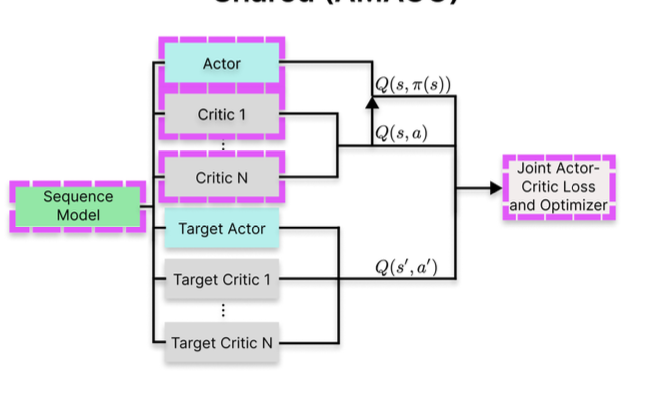
\includegraphics[height=1.5in]{figs/amago}
    \caption{
      The Amago actor-critic model.
      Purple boxes are involved in training.
      The green box is a the slow-to-train transformer backbone.
      The blue actor and gray critics are lightweight feedforward
      output heads.
\figtaken{Figure 10 if \citep{Grigsby2024}}.
}
\label{fig:amago}
\end{figure}

The recent  \keywordDef{Amago} algorithm \citep{Grigsby2024}
modifies the discrete SAC algorithm by considering  $\alpha=0$;
they  end up with a learning rule similar to DDPG (\cref{sec:DDPQ}).
In more detail,
%let $\vq_s = [Q(s,a_1),\ldots,Q(s,a_K)]$ be a vector
%of $Q$ values for each possible action, and let
%$\vmu_s = [\pi(a_1|s), \ldots, \pi(a_K|s)]$ be a vector
%of action probabilities.
let $\overline{Q}$ and $\overline{\pi}$ represent the frozen
(target) values of these functions, derived from EMA.
The critic loss can be written as an average
of the following loss, where we sample tuples from the replay buffer:
\be
  \loss_{\text{TD}}(\vs,a,r,\vs') = (Q(\vs,a) - (r+\gamma
    \stopgrad(\overline{V}(\vs,a)))^2 
  \ee
where the  value function is given by
\begin{align}
  \overline{V}(\vs) &=
  \sum_a \overline{\pi}(a|\vs) \overline{Q}(\vs,a)
  \end{align}
The actor  loss
(which we want to minimize, so negative of the previous objective)
is given by an average of the following loss,
where we sample states from the replay buffer:
\begin{align}
  \loss_{\text{PG}}(\vs) &= -\sum_a    \pi(a|\vs) Q(\vs,a)
\end{align}

In the limit that the policy becomes deterministic,
the value function becomes
\be
\overline{V}(\vs,a) = \overline{Q}(\vs,\overline{\pi}(\vs))
\ee
which is plugged into the critic loss.
The actor loss becomes 
\begin{align}
  \loss_{\text{PG}}(\vs)=-Q(\vs, \pi(\vs))
\end{align}
This gives an update similar to DDPQ.
Note that exploration can be ensured by using
a method such as epsilon-greedy, even if the policy is deterministic.
%Furthermore, the policy network still learns a distribution,
%which can be sampled from.

The actor and critic are both defined in terms of a shared
transformer sequence model,
with different output heads. (In fact they  have $N$ output heads
for the different $Q$ functions, as in REDQ, and maintain
a target version of the policy and the $N$ critics,
as shown in \cref{fig:amago}.
To train the shared model, they 
 construct a unified objective
$\loss = E[\lambda_0 \loss_{TD} + \lambda_1 \loss_{PG}]$,
where the TD and policy gradient losses are dynamically normalized
using the \keywordDef{PopArt} method
of \citep{van-Hasselt2016,Hessel2019}
to allow
for a fixed set of hyper-parameter values for $\lambda_i$,
even as the range of the losses change over time.
%(PopArt  stands for
%``Preserving Outputs Precisely, while Adaptively Rescaling Targets''.)
They show good results on challenging environments such as MineCraft.

}

\eat{
  
Yes, the discrete version is implemented like SAC-Discrete, where the actor outputs a softmax over actions, and the critic uses that distribution to reduce variance. In my experience, the main benefit of SAC's entropy is that it smooths TD targets in the critic update (similar to the manual noise of TD3) rather than the exploration improvement it's usually motivated by. When another technique is already stabilizing the critic update, it reduces tuning to remove entropy constraints and ensure exploration with a more intuitive epsilon-greedy schedule.

AMAGO has a second actor term that does weighted max likelihood on actions from the buffer. This is the main reason we need the actor network for discrete environments rather than taking the argmax over the critic like DQN variants. It also makes the discrete and continuous versions very similar. The second loss term is a safety measure for when the critic is inaccurate, as it essentially reduces the update to supervised learning with a Transformer. This turns out to be more important for multi-task problems than we thought and we're about to release a follow-up paper about it.

The update has the same theoretical properties as DDPG in an MDP
because the policy is allowed to become deterministic if that turns
out to be optimal. In meta-RL/POMDPs we’d rather be able to learn a
stochastic policy when the model has finite memory length, and we
always sample during evaluation.
}







\section{Deterministic policy gradient methods}
\label{sec:DPG}

In this section, we consider the case of a deterministic
policy, that predicts a unique action for each state,
so $a_t = \policydet(s_t)$,
rather than $a_t \sim \polapprox(s_t)$.
(We require that the actions are continuous,
because we will take the Jacobian of the $Q$ function
wrt the actions; if the actions are discrete,
we can just use DQN.)
The advantage of using a deterministic policy
is that we can modify the policy gradient method
so that it can work off policy without
needing importance sampling, as we will see.


Following
\cref{eqn:JJpi},
we define the value of a policy as the expected discounted
reward per state:
\begin{align}
\polval(\policydet)
%= \int_S \statdistdet(s) R(s, \policydet(s)) ds
\defeq  \expectQ{R(s,\policydet(s))}{\statmeasuredet(s)}
\end{align}
The \keywordDef{deterministic policy gradient theorem}
\citep{dpg} tells us that the gradient of this expression
is given by
\begin{align}
\nabla_{\vtheta} \polval(\policydet)
&=  \expectQ{\nabla_{\vtheta} \Qdet(s,
  \policydet(s))}
      {\statmeasuredet(s)} \\
&= \expectQ{\nabla_{\vtheta} \policydet(s)
 \nabla_a \Qdet(s, a)|_{a=\policydet(s)}}{\statmeasuredet(s)}
\label{eqn:DDPGgrad}
\end{align}
where $\nabla_{\vtheta} \policydet(s)$ is
the $M \times N$ Jacobian matrix,
and $M$ and $N$ are the dimensions
of $\calA$ and $\vtheta$, respectively.
%the number of action dimensions,
%and $N$ is the number of policy parameters.
For stochastic policies of the form
$\polapprox(a|s) = \policydet(s) + \text{noise}$,
the standard policy gradient theorem reduces
to the above form as the noise level goes to zero.

Note that the gradient estimate
in \cref{eqn:DDPGgrad}
integrates over the states but not over the actions,
which helps reduce the variance in gradient estimation
from sampled trajectories.
However, since the deterministic policy does not do any exploration,
we need to use an \keyword{off-policy method} for training.
This collects data from 
a stochastic behavior policy $\behavior$,
whose stationary state distribution is
$\statdistbehave$.
%We define the objective in a similar way to \cref{eqn:offPolicyJ}:
The original objective, $\polval(\policydet)$, is approximated by the following:
\begin{align}
\polvalbeh(\policydet)
\defeq \expectQ{\Vdet(s)}{\statdistbehave(s)}
= \expectQ{\Qdet(s, \policydet(s))}{\statdistbehave(s)}
\end{align}
with the off-policy deterministic policy gradient
from \citep{Degris2012}
is approximated by
%(see also \cref{sec:offpolicyRL-IS})
\begin{align}
\label{eqn:OffDDPGgrad}
\nabla_{\vtheta} \polvalbeh(\policydet)
\approx \expectQ{\nabla_{\vtheta} \left[\Qdet(s,
    \policydet(s))\right]}
        {\statdistbehave(s)}
= \expectQ{\nabla_{\vtheta} \policydet(s)
 \nabla_a \Qdet(s, a)|_{a=\policydet(s)}  }{\statdistbehave(s)}
\end{align}
where we have a dropped a term that depends on
$\nabla_{\vtheta} \Qdet(s,a)$ and is hard to estimate
\citep{dpg}.

To apply \cref{eqn:OffDDPGgrad}, we may learn $\Qapprox \approx \Qdet$ with TD,
giving rise to the following updates:
\begin{align}
\delta &= r_t + \gamma \Qapprox(s_{t+1}, \policydet(s_{t+1}))
- \Qapprox(s_t, a_t) \\
\vw_{t+1} &\assign \vw_t + \lr_{\vw} \delta \nabla_{\vw} \Qapprox(s_t,a_t) \\
\vtheta_{t+1} &\assign \vtheta_t + \lr_{\vtheta} \nabla_{\vtheta} \policydet(s_t)
\nabla_a \Qapprox(s_t,a)|_{a=\policydet(s_t)} 
\end{align}
So we learn both a state-action critic $Q_{\vw}$
and an actor $\vmu_{\vtheta}$.
This method avoids importance sampling
in the actor update because
of the deterministic policy gradient,
and we avoids it  in the critic
update because of the use of Q-learning.

If $\Qapprox$ is linear in $\vw$, and uses features
of the form $\vphi(s,a) = \va^\trans \nabla_{\vtheta} \policydet(s)$,
%where $\va$ is the vector representation of $a$,
then we say the function approximator for the critic
is \keywordDef{compatible} with the actor;
in this case, one can show that the above approximation
does not bias the overall gradient.
%Of course, this is rather restrictive.

%https://www.reddit.com/r/reinforcementlearning/comments/fafi7j/actorcritic_for_discrete_action_space/

The basic off-policy
DPG method has been extended in various ways,
some of which we describe below.

\subsection{DDPG}
\label{sec:DDPG}
\label{sec:D4PG}


The \keywordDef{DDPG} algorithm of \citep{ddpg},
which stands for
``\keyword{deep deterministic policy gradient}'',
uses  the DQN method (\cref{sec:DQN})
to update $Q$ that is represented by deep neural networks.
%
In more detail, the actor tries to minimize the output of the critic
by optimize
\be
\loss_{\vtheta}(s) = Q_{\vw}(s, \mu_{\vtheta}(s))
\ee
averaged over states $s$ drawn from the replay buffer.
The  critic tries to minimize
the 1-step TD loss
\be
\loss_{\vw}(s,a,r,s') =
[Q_{\vw}(s,a) - (r + \gamma Q_{\overline{\vw}}(s',\mu_{\vtheta}(s')))]^2
\ee
where $Q_{\overline{\vw}}$ is the target critic network,
and the samples $(s,a,r,a')$ are drawn from a replay buffer.
(See \cref{sec:targetNetwork} for a discussion of target networks.)

The \keywordDef{D4PG} algorithm \citep{D4PG},
which stands for ``distributed distributional DDPG'',
extends DDPG to
handle distributed training,
and to handle \keyword{distributional RL}
(see \cref{sec:distributional}).


\subsection{Twin Delayed DDPG (TD3)}
\label{sec:TD3}

The  \keywordDef{TD3} (``twin delayed deep deterministic'') method of
\citep{TD3}
extends DDPG  in 3 main ways.
First, it uses \keywordDef{target policy smoothing},
in which noise is added to the action, to encourage generalization:
\be
\tilde{\va} = \vmu_{\vtheta}(\vs) + \text{noise}
= \pi_{\vtheta}(\vs)
\ee
Second it uses \keywordDef{clipped double Q learning},
which is an extension of the double Q-learning discussed in
\cref{sec:double} to avoid
over-estimation bias.
In particular, the target values for TD learning are defined using
\be
\TargetV(r,\vs'; \overline{\vw}_{1:2}, \overline{\vtheta})
= r + \gamma \min_{i=1,2}
Q_{\overline{\vw}_i}(\vs', \pi_{\overline{\vtheta}}(\vs'))
\ee
Third, it uses \keywordDef{delayed policy updates},
in which it only updates the policy after the value function
has stabilized. (See also \cref{sec:bilevel}.)
See \cref{algo:TD3} for the pseudcode.


\begin{algorithm}
\dontprintsemicolon
\caption{TD3}
\label{algo:TD3}
Initialize environment state $\vs$,
policy parameters $\vtheta$,
target policy parameters $\overline{\vtheta}$,
critic parameters $\vw_i$,
target critic parameters $\overline{\vw}_i = \vw_i$,
replay buffer $\data=\emptyset$,
discount factor $\gamma$,
EMA rate $\rho$,
step size $\lr_{\vw}$, $\lr_{\vtheta}$.
\\
\Repeat{converged}
       {
         $\va = \mu_{\vtheta}(\vs) + \text{noise}$ \\
         $(\vs',r) = \text{step}(\va, \vs)$ \\
         $\data := \data \union
         \{ (\vs, \va, r, \vs') \}$ \\
         $\vs \assign \vs'$ \\
         \For{$G$ updates}{
         Sample a minibatch $\calB = \{(\vs_j,\va_j,r_j,\vs'_j)\}$
         from $\data$ \\
           $\vw = \text{update-critics}(\vtheta, \vw, \calB)$
         }
         Sample a minibatch $\calB = \{(\vs_j,\va_j,r_j,\vs'_j)\}$
         from $\data$\\
         $\vtheta = \text{update-policy}(\vtheta,\vw, \calB)$
        }
.\\
$\text{def update-critics}(\vtheta,\vw,\calB)$: \\
       Let $(\vs_j,\va_j,r_j,\vs'_j)_{j=1}^B = \calB$ \\
       \For{$j=1:B$}{
         $\tilde{\va}_j = \mu_{\overline{\vtheta}}(\vs'_j)
         + \text{clip}(\text{noise}, -c, c)$ \\
         $\targetV_j = r_j + \gamma \min_{i=1,2} Q_{\overline{\vw}_i}(\vs'_j,
         \tilde{\va}_j)$
       }
       \For{$i=1:2$}
    {
      $\loss(\vw_i) = \frac{1}{|\calB|} \sum_{(\vs,\va,r,\vs')_j \in
        \calB} (Q_{\vw_i}(\vs_j,\va_j) - \stopgrad(\targetV_j))^2$\\
      $\vw_i \assign \vw_i - \lr_{\vw} \nabla \loss(\vw_i)$ // Descent
      \\
      $\overline{\vw}_i := \rho \overline{\vw}_i
      + (1-\rho) \vw_i$       //Update target networks with EMA\\
    }

    Return $\vw_{1:N}, \overline{\vw}_{1:N}$\\
.\\
$\text{def update-actor}(\vtheta,\vw,\calB)$: \\
$J(\vtheta) =
 \frac{1}{|\calB|} \sum_{\vs \in \calB}
 \left(Q_{\vw_1}(\vs, \mu_{\vtheta}(\vs)) \right)^2$ \\
 $\vtheta \assign \vtheta +  \lr_{\vtheta} \nabla J(\vtheta)$ //
 Ascent \\
       $\overline{\vtheta} := \rho \overline{\vtheta}
       + (1-\rho) \vtheta$       //Update target policy network with EMA \\
         Return $\vtheta, \overline{\vtheta}$
\end{algorithm}






\eat{
\section{Gradient-free methods}
\label{sec:PGrnd}

The policy gradient
estimator computes a ``zeroth order'' gradient, which essentially
evaluates the function with randomly sampled trajectories.
Sometimes it can be more efficient to
use a derivative-free optimizer (\cref{sec:DFO}),
that does not even attempt to estimate the gradient.
For example, \citep{Mania2018} obtain good results
by training linear policies with random search,
and \citep{Salimans2017ES} show how to use
evolutionary strategies to optimize the policy
of a robotic controller.
}
